% Options for packages loaded elsewhere
\PassOptionsToPackage{unicode}{hyperref}
\PassOptionsToPackage{hyphens}{url}
%
\documentclass[
  oneside,
  open=any]{scrbook}

\usepackage{amsmath,amssymb}
\usepackage{iftex}
\ifPDFTeX
  \usepackage[T1]{fontenc}
  \usepackage[utf8]{inputenc}
  \usepackage{textcomp} % provide euro and other symbols
\else % if luatex or xetex
  \usepackage{unicode-math}
  \defaultfontfeatures{Scale=MatchLowercase}
  \defaultfontfeatures[\rmfamily]{Ligatures=TeX,Scale=1}
\fi
\usepackage{lmodern}
\ifPDFTeX\else  
    % xetex/luatex font selection
\fi
% Use upquote if available, for straight quotes in verbatim environments
\IfFileExists{upquote.sty}{\usepackage{upquote}}{}
\IfFileExists{microtype.sty}{% use microtype if available
  \usepackage[]{microtype}
  \UseMicrotypeSet[protrusion]{basicmath} % disable protrusion for tt fonts
}{}
\makeatletter
\@ifundefined{KOMAClassName}{% if non-KOMA class
  \IfFileExists{parskip.sty}{%
    \usepackage{parskip}
  }{% else
    \setlength{\parindent}{0pt}
    \setlength{\parskip}{6pt plus 2pt minus 1pt}}
}{% if KOMA class
  \KOMAoptions{parskip=half}}
\makeatother
\usepackage{xcolor}
\setlength{\emergencystretch}{3em} % prevent overfull lines
\setcounter{secnumdepth}{5}
% Make \paragraph and \subparagraph free-standing
\ifx\paragraph\undefined\else
  \let\oldparagraph\paragraph
  \renewcommand{\paragraph}[1]{\oldparagraph{#1}\mbox{}}
\fi
\ifx\subparagraph\undefined\else
  \let\oldsubparagraph\subparagraph
  \renewcommand{\subparagraph}[1]{\oldsubparagraph{#1}\mbox{}}
\fi
\usepackage{color}
\usepackage{fancyvrb}
\newcommand{\VerbBar}{|}
\newcommand{\VERB}{\Verb[commandchars=\\\{\}]}
\DefineVerbatimEnvironment{Highlighting}{Verbatim}{commandchars=\\\{\}}
% Add ',fontsize=\small' for more characters per line
\usepackage{framed}
\definecolor{shadecolor}{RGB}{241,243,245}
\newenvironment{Shaded}{\begin{snugshade}}{\end{snugshade}}
\newcommand{\AlertTok}[1]{\textcolor[rgb]{0.68,0.00,0.00}{#1}}
\newcommand{\AnnotationTok}[1]{\textcolor[rgb]{0.37,0.37,0.37}{#1}}
\newcommand{\AttributeTok}[1]{\textcolor[rgb]{0.40,0.45,0.13}{#1}}
\newcommand{\BaseNTok}[1]{\textcolor[rgb]{0.68,0.00,0.00}{#1}}
\newcommand{\BuiltInTok}[1]{\textcolor[rgb]{0.00,0.23,0.31}{#1}}
\newcommand{\CharTok}[1]{\textcolor[rgb]{0.13,0.47,0.30}{#1}}
\newcommand{\CommentTok}[1]{\textcolor[rgb]{0.37,0.37,0.37}{#1}}
\newcommand{\CommentVarTok}[1]{\textcolor[rgb]{0.37,0.37,0.37}{\textit{#1}}}
\newcommand{\ConstantTok}[1]{\textcolor[rgb]{0.56,0.35,0.01}{#1}}
\newcommand{\ControlFlowTok}[1]{\textcolor[rgb]{0.00,0.23,0.31}{#1}}
\newcommand{\DataTypeTok}[1]{\textcolor[rgb]{0.68,0.00,0.00}{#1}}
\newcommand{\DecValTok}[1]{\textcolor[rgb]{0.68,0.00,0.00}{#1}}
\newcommand{\DocumentationTok}[1]{\textcolor[rgb]{0.37,0.37,0.37}{\textit{#1}}}
\newcommand{\ErrorTok}[1]{\textcolor[rgb]{0.68,0.00,0.00}{#1}}
\newcommand{\ExtensionTok}[1]{\textcolor[rgb]{0.00,0.23,0.31}{#1}}
\newcommand{\FloatTok}[1]{\textcolor[rgb]{0.68,0.00,0.00}{#1}}
\newcommand{\FunctionTok}[1]{\textcolor[rgb]{0.28,0.35,0.67}{#1}}
\newcommand{\ImportTok}[1]{\textcolor[rgb]{0.00,0.46,0.62}{#1}}
\newcommand{\InformationTok}[1]{\textcolor[rgb]{0.37,0.37,0.37}{#1}}
\newcommand{\KeywordTok}[1]{\textcolor[rgb]{0.00,0.23,0.31}{#1}}
\newcommand{\NormalTok}[1]{\textcolor[rgb]{0.00,0.23,0.31}{#1}}
\newcommand{\OperatorTok}[1]{\textcolor[rgb]{0.37,0.37,0.37}{#1}}
\newcommand{\OtherTok}[1]{\textcolor[rgb]{0.00,0.23,0.31}{#1}}
\newcommand{\PreprocessorTok}[1]{\textcolor[rgb]{0.68,0.00,0.00}{#1}}
\newcommand{\RegionMarkerTok}[1]{\textcolor[rgb]{0.00,0.23,0.31}{#1}}
\newcommand{\SpecialCharTok}[1]{\textcolor[rgb]{0.37,0.37,0.37}{#1}}
\newcommand{\SpecialStringTok}[1]{\textcolor[rgb]{0.13,0.47,0.30}{#1}}
\newcommand{\StringTok}[1]{\textcolor[rgb]{0.13,0.47,0.30}{#1}}
\newcommand{\VariableTok}[1]{\textcolor[rgb]{0.07,0.07,0.07}{#1}}
\newcommand{\VerbatimStringTok}[1]{\textcolor[rgb]{0.13,0.47,0.30}{#1}}
\newcommand{\WarningTok}[1]{\textcolor[rgb]{0.37,0.37,0.37}{\textit{#1}}}

\providecommand{\tightlist}{%
  \setlength{\itemsep}{0pt}\setlength{\parskip}{0pt}}\usepackage{longtable,booktabs,array}
\usepackage{calc} % for calculating minipage widths
% Correct order of tables after \paragraph or \subparagraph
\usepackage{etoolbox}
\makeatletter
\patchcmd\longtable{\par}{\if@noskipsec\mbox{}\fi\par}{}{}
\makeatother
% Allow footnotes in longtable head/foot
\IfFileExists{footnotehyper.sty}{\usepackage{footnotehyper}}{\usepackage{footnote}}
\makesavenoteenv{longtable}
\usepackage{graphicx}
\makeatletter
\def\maxwidth{\ifdim\Gin@nat@width>\linewidth\linewidth\else\Gin@nat@width\fi}
\def\maxheight{\ifdim\Gin@nat@height>\textheight\textheight\else\Gin@nat@height\fi}
\makeatother
% Scale images if necessary, so that they will not overflow the page
% margins by default, and it is still possible to overwrite the defaults
% using explicit options in \includegraphics[width, height, ...]{}
\setkeys{Gin}{width=\maxwidth,height=\maxheight,keepaspectratio}
% Set default figure placement to htbp
\makeatletter
\def\fps@figure{htbp}
\makeatother
% definitions for citeproc citations
\NewDocumentCommand\citeproctext{}{}
\NewDocumentCommand\citeproc{mm}{%
  \begingroup\def\citeproctext{#2}\cite{#1}\endgroup}
\makeatletter
 % allow citations to break across lines
 \let\@cite@ofmt\@firstofone
 % avoid brackets around text for \cite:
 \def\@biblabel#1{}
 \def\@cite#1#2{{#1\if@tempswa , #2\fi}}
\makeatother
\newlength{\cslhangindent}
\setlength{\cslhangindent}{1.5em}
\newlength{\csllabelwidth}
\setlength{\csllabelwidth}{3em}
\newenvironment{CSLReferences}[2] % #1 hanging-indent, #2 entry-spacing
 {\begin{list}{}{%
  \setlength{\itemindent}{0pt}
  \setlength{\leftmargin}{0pt}
  \setlength{\parsep}{0pt}
  % turn on hanging indent if param 1 is 1
  \ifodd #1
   \setlength{\leftmargin}{\cslhangindent}
   \setlength{\itemindent}{-1\cslhangindent}
  \fi
  % set entry spacing
  \setlength{\itemsep}{#2\baselineskip}}}
 {\end{list}}
\usepackage{calc}
\newcommand{\CSLBlock}[1]{\hfill\break\parbox[t]{\linewidth}{\strut\ignorespaces#1\strut}}
\newcommand{\CSLLeftMargin}[1]{\parbox[t]{\csllabelwidth}{\strut#1\strut}}
\newcommand{\CSLRightInline}[1]{\parbox[t]{\linewidth - \csllabelwidth}{\strut#1\strut}}
\newcommand{\CSLIndent}[1]{\hspace{\cslhangindent}#1}

\usepackage{tabularx, lipsum}
\usepackage{color,soul}
\makeatletter
\@ifpackageloaded{caption}{}{\usepackage{caption}}
\AtBeginDocument{%
\ifdefined\contentsname
  \renewcommand*\contentsname{Table of contents}
\else
  \newcommand\contentsname{Table of contents}
\fi
\ifdefined\listfigurename
  \renewcommand*\listfigurename{List of Figures}
\else
  \newcommand\listfigurename{List of Figures}
\fi
\ifdefined\listtablename
  \renewcommand*\listtablename{List of Tables}
\else
  \newcommand\listtablename{List of Tables}
\fi
\ifdefined\figurename
  \renewcommand*\figurename{Figure}
\else
  \newcommand\figurename{Figure}
\fi
\ifdefined\tablename
  \renewcommand*\tablename{Table}
\else
  \newcommand\tablename{Table}
\fi
}
\@ifpackageloaded{float}{}{\usepackage{float}}
\floatstyle{ruled}
\@ifundefined{c@chapter}{\newfloat{codelisting}{h}{lop}}{\newfloat{codelisting}{h}{lop}[chapter]}
\floatname{codelisting}{Listing}
\newcommand*\listoflistings{\listof{codelisting}{List of Listings}}
\makeatother
\makeatletter
\makeatother
\makeatletter
\@ifpackageloaded{caption}{}{\usepackage{caption}}
\@ifpackageloaded{subcaption}{}{\usepackage{subcaption}}
\makeatother

\usepackage{hyphenat}
\usepackage{ifthen}
\usepackage{calc}
\usepackage{calculator}

\usepackage{graphicx}
\usepackage{wallpaper}

\usepackage{geometry}

\usepackage{graphicx}
\usepackage{geometry}
\usepackage{afterpage}
\usepackage{tikz}
\usetikzlibrary{calc}
\usetikzlibrary{fadings}
\usepackage[pagecolor=none]{pagecolor}


% Set the titlepage font families







% Set the coverpage font families

\ifLuaTeX
  \usepackage{selnolig}  % disable illegal ligatures
\fi
\usepackage{bookmark}

\IfFileExists{xurl.sty}{\usepackage{xurl}}{} % add URL line breaks if available
\urlstyle{same} % disable monospaced font for URLs
\hypersetup{
  pdftitle={Cataloguing and visualizing big Geodata},
  pdfauthor={Martín Domínguez Durán},
  hidelinks,
  pdfcreator={LaTeX via pandoc}}

\title{Cataloguing and visualizing big Geodata}
\usepackage{etoolbox}
\makeatletter
\providecommand{\subtitle}[1]{% add subtitle to \maketitle
  \apptocmd{\@title}{\par {\large #1 \par}}{}{}
}
\makeatother
\subtitle{Final report}
\author{Martín Domínguez Durán}
\date{}

\begin{document}
%%%%% begin titlepage extension code

  \begin{frontmatter}

\begin{titlepage}

%%% TITLE PAGE START

% Set up alignment commands
%Page
\newcommand{\titlepagepagealign}{
\ifthenelse{\equal{left}{right}}{\raggedleft}{}
\ifthenelse{\equal{left}{center}}{\centering}{}
\ifthenelse{\equal{left}{left}}{\raggedright}{}
}


\newcommand{\titleandsubtitle}{
% Title and subtitle
{{\large{\bfseries{\nohyphens{Cataloguing and visualizing big
Geodata}}}}\par
}%

\vspace{\betweentitlesubtitle}
{
{\large{\textit{\nohyphens{Final report}}}}\par
}}
\newcommand{\titlepagetitleblock}{
\titleandsubtitle
}

\newcommand{\authorstyle}[1]{{\large{#1}}}

\newcommand{\affiliationstyle}[1]{{\large{#1}}}

\newcommand{\titlepageauthorblock}{
{\authorstyle{\nohyphens{Martín Domínguez Durán}{\textsuperscript{1}}}}}

\newcommand{\titlepageaffiliationblock}{
\hangindent=1em
\hangafter=1
{\affiliationstyle{
{1}.~Wageningen University \& Research,~Wageningen, The Netherlands


\vspace{1\baselineskip} 
}}
}
\newcommand{\headerstyled}{%
{The Publisher}
}
\newcommand{\footerstyled}{%
{\large{\textbf{Registration number:} 1254246\\
\textbf{Period of Internship:} 2024-04-08 - 2024-08-08\\
\textbf{Date final report:} 2024-07-31\\
\textbf{Telephone number student:} +31651120353\\
\textbf{Name of Company:} Satelligence B.V.\\
\textbf{Host supervisor:} Luca Foresta\\
\textbf{MGI supervisor:} Lukasz Grus}}
}
\newcommand{\datestyled}{%
{}
}


\newcommand{\titlepageheaderblock}{\headerstyled}

\newcommand{\titlepagefooterblock}{
\footerstyled
}

\newcommand{\titlepagedateblock}{
\datestyled
}

%set up blocks so user can specify order
\newcommand{\titleblock}{\newlength{\betweentitlesubtitle}
\setlength{\betweentitlesubtitle}{\baselineskip}
{

{\titlepagetitleblock}
}

\vspace{4\baselineskip}
}

\newcommand{\authorblock}{{\titlepageauthorblock}

\vspace{2\baselineskip}
}

\newcommand{\affiliationblock}{{\titlepageaffiliationblock}

\vspace{1pt}
}

\newcommand{\logoblock}{{
\includegraphics[width=0.7\textheight]{img/logo.png}}

\vspace{2\baselineskip}
}

\newcommand{\footerblock}{{\titlepagefooterblock}

\vspace{1pt}
}

\newcommand{\dateblock}{}

\newcommand{\headerblock}{{\titlepageheaderblock

\vspace{0pt}
}}
\newgeometry{top=3in,bottom=1in,right=1in,left=1in}
% background image
\newlength{\bgimagesize}
\setlength{\bgimagesize}{0.5\paperwidth}
\LENGTHDIVIDE{\bgimagesize}{\paperwidth}{\theRatio} % from calculator pkg
\ThisULCornerWallPaper{\theRatio}{img/corner-bg.png}

\thispagestyle{empty} % no page numbers on titlepages


\newcommand{\vrulecode}{\rule{\vrulewidth}{\textheight}}
\newlength{\vrulewidth}
\setlength{\vrulewidth}{1pt}
\newlength{\B}
\setlength{\B}{\ifdim\vrulewidth > 0pt 0.05\textwidth\else 0pt\fi}
\newlength{\minipagewidth}
\ifthenelse{\equal{left}{left} \OR \equal{left}{right} }
{% True case
\setlength{\minipagewidth}{\textwidth - \vrulewidth - \B - 0.1\textwidth}
}{
\setlength{\minipagewidth}{\textwidth - 2\vrulewidth - 2\B - 0.1\textwidth}
}
\ifthenelse{\equal{left}{left} \OR \equal{left}{leftright}}
{% True case
\raggedleft % needed for the minipage to work
\vrulecode
\hspace{\B}
}{%
\raggedright % else it is right only and width is not 0
}
% [position of box][box height][inner position]{width}
% [s] means stretch out vertically; assuming there is a vfill
\begin{minipage}[b][\textheight][s]{\minipagewidth}
\titlepagepagealign
\titleblock

\authorblock

\affiliationblock

\vfill

\logoblock

\footerblock
\par

\end{minipage}\ifthenelse{\equal{left}{right} \OR \equal{left}{leftright} }{
\hspace{\B}
\vrulecode}{}
\clearpage
\restoregeometry
%%% TITLE PAGE END
\end{titlepage}
\setcounter{page}{1}
\end{frontmatter}

%%%%% end titlepage extension code

\renewcommand*\contentsname{Table of contents}
{
\setcounter{tocdepth}{2}
\tableofcontents
}
\listoffigures
\mainmatter
\chapter*{Executive summary}\label{executive-summary}
\addcontentsline{toc}{chapter}{Executive summary}

\lipsum[100]

\newpage

\chapter*{List of abreviations}\label{list-of-abreviations}
\addcontentsline{toc}{chapter}{List of abreviations}

\begin{longtable}[]{@{}
  >{\raggedright\arraybackslash}p{(\columnwidth - 2\tabcolsep) * \real{0.5556}}
  >{\raggedright\arraybackslash}p{(\columnwidth - 2\tabcolsep) * \real{0.4444}}@{}}
\caption{Abbreviation list}\tabularnewline
\toprule\noalign{}
\begin{minipage}[b]{\linewidth}\raggedright
\textbf{Abreviations}
\end{minipage} & \begin{minipage}[b]{\linewidth}\raggedright
\textbf{Description}
\end{minipage} \\
\midrule\noalign{}
\endfirsthead
\toprule\noalign{}
\begin{minipage}[b]{\linewidth}\raggedright
\textbf{Abreviations}
\end{minipage} & \begin{minipage}[b]{\linewidth}\raggedright
\textbf{Description}
\end{minipage} \\
\midrule\noalign{}
\endhead
\bottomrule\noalign{}
\endlastfoot
EUDR & European Union Deforestation Regulation \\
STAC & Spatio-Temporal Asset Catalog \\
COG & Cloud-Optimized GeoTiff \\
OGC & Open Geospatial Consortium \\
SDI & Spatial Data Infrastructure \\
S11 & Satelligence \\
K8 & Kubernetes \\
DPROF & Distributed Processing Framework \\
JSON & JavaScript Object Notation \\
API & Application Programming Interfaces \\
HTTP & HyperText Transfer Protocol \\
SQL & Standard Query Language \\
FBL & Forest Baseline \\
DEM & Digital Elevation Map \\
TCA & Thematic Content analysis \\
VRT & Vitual Raster \\
\end{longtable}

\chapter{Introduction}\label{introduction}

\section{Internship organization
background}\label{internship-organization-background}

Satelligence (S11) is a company founded in 2016 that specializes in
providing satellite-based actionable information by monitoring
environmental risks in commodity supply chains and financial investment
planning (\citeproc{ref-satelligence_home_nodate}{Satelligence, n.d.}).
More specifically, the company processes terabytes of satellite imagery
to detect environmental risks and presents this information to their
clients in a web application to assist them in the migration towards
more sustainable sourcing models and the compliance with
deforestation-free commodities regulations, such as the European Union
Deforestation Regulation (EUDR)
(\citeproc{ref-satelligence_internship_2023}{Satelligence, 2023}). S11's
main focus is continuous deforestation monitoring (CDM) in the tropics
using freely accessible satellite imagery. This is a data-intensive task
that is achieved by leveraging the benefits of cloud computing,
specifically Google Cloud Platform.

\section{Context and justification of
research}\label{context-and-justification-of-research}

Satelligence strongly relies on cloud computing for their services. They
process extensive volumes of satellite imagery amounting to terabytes
using DPROF, a distributed processing framework created within the
company to efficiently process multidimensional spatial datasets. While
this processing workflow currently runs smoothly, the company's data and
operations teams face challenges when going deeper into the analysis and
accessing intermediate results due to the big nature of this data
(\citeproc{ref-satelligence_internship_2023}{Satelligence, 2023}).
Scholars have defined big data as datasets characterized by their high
Volume, Velocity, and Variety, which makes it paramount to use advanced
processing and analytics techniques to derive relevant insights
(\citeproc{ref-giri_big_2014}{Giri and Lone, 2014}). In the specific
case of Satelligence, their datasets can be categorized as big data due
to their: High volume (Terabytes of satellite images processed every
day), high velocity (Near -- real time processing of these images) and
high variety (Imagery coming from different sensors and regions). All
these datasets are a specific case of big data: Big Geodata.

\subsection{Significance of the topic and previous
research}\label{significance-of-the-topic-and-previous-research}

In the past decades there has been a rapid increase in the amount and
size of geo-spatial information that can be accessed. Nowadays, more
than 150 satellites orbit the earth collecting thousands of images every
single day (\citeproc{ref-zhao_scalable_2021}{Zhao et al., 2021}). This
has made data handling and the introduction of spatial data
infrastructures (SDIs) paramount when working with such big datasets.

Traditionally, SDIs have served to ease the accessibility, integration
and analysis of spatial data
(\citeproc{ref-rajabifard_spatial_2001}{Rajabifard and Williamson,
2001}). However, in practice SDIs have been built upon technologies that
focus on data preservation rather than accessibility
(\citeproc{ref-durbha_advances_2023}{Durbha et al., 2023}). Due to this,
an important shift is underway towards more cloud-based SDIs
(\citeproc{ref-tripathi_cloud_2020}{Tripathi et al., 2020}). These
platforms need the emergence of new technologies that prioritize
seamless access to cloud-stored data, efficient discovery services that
ensure the easy location of extensive spatial data, and data
visualization interfaces where multiple datasets can be depicted.

\subsubsection*{Cloud-based data
storage}\label{cloud-based-data-storage}
\addcontentsline{toc}{subsubsection}{Cloud-based data storage}

Spatial data, just like any other type of data, can be cataloged into
structured and unstructured data. Structured datasets are often
organized and follow a specific structure (i.e.~A traditional table with
rows (objects) and columns (features)). On the other hand, unstructured
data does not have a predefined structure (e.g.~Satellite imagery and
Time series data) (\citeproc{ref-mishra_structured_2017}{Mishra and
Misra, 2017}). The management of structured data has witnessed
substantial advancements, making it straightforward to handle it
systematically using, for instance, relational databases (i.e.~With the
help of Structured Query Language (SQL))
(\citeproc{ref-kaufmann_database_2023}{Kaufmann and Meier, 2023}). In
contrast, due to the additional challenges associated with the handling
of unstructured data, the developments in this area have taken a longer
time to appear.

The emergence of cloud-based archives has been one of the main
advancements for unstructured data management during the last decades.
In the specific case of geo-spatial data, it has allowed to store
terabytes of unstructured data (i.e.~Satellite imagery) on the cloud and
access it through the network. However, the necessity transmitting data
across networks to access it makes it essential to develop new data
formats suited for such purposes
(\citeproc{ref-durbha_advances_2023}{Durbha et al., 2023}).

At S11, the storage of large geo-spatial data is already managed using
Google Storage Buckets, and they are currently in the process of
incorporating the conversion to cloud-optimized data formats like Cloud
Optimized GeoTIFFs (COGs) and Zarrs in their processing framework
(DPROF) to improve efficiency and accessibility.

\newpage

\textbf{Cloud-optimized data formats}

\emph{COG}

Cloud-Optimized GeoTIFFs (\href{https://www.cogeo.org/}{COGs}) are an
example of data formats that have been created to ease the access of
data stored in the cloud. They improve the readability by including the
metadata in the initial bytes of the file stored, storing different
image overviews for different scales and tiling the images in smaller
blocks. These characteristics make COG files heavier than traditional
image formats. However, they also greatly enhance accessibility by
enabling the selective transfer of only the necessary tiles using HTTP
GET requests (\citeproc{ref-desruisseaux_ogc_2021}{Desruisseaux et al.,
2021}). Additionally, this data format has been adopted as an Open
Geospatial Consortium (OGC) standard. These standards are a set of
guidelines and specifications created to facilitate data
interoperability (\citeproc{ref-ogc_ogc_2023}{OGC, 2023}).

\emph{Zarr}

Another cloud native data format that has gained popularity recently is
\href{https://zarr.readthedocs.io/en/stable/}{Zarr}. This data format
and python library focuses on the cloud-optimization of n-dimensional
arrays. Zarr, differently than COGs store the metadata separately from
the data chunks using lightweight external JSON files
(\citeproc{ref-durbha_advances_2023}{Durbha et al., 2023}).
Additionally, this data format stores the N-dimensional arrays in
smaller chunks that can be accessed more easily. While the storage of
Zarr files in chunks facilitates more efficient data access, the absence
of overviews hinders the visualization of this data in a web map service
(\citeproc{ref-desruisseaux_ogc_2021}{Desruisseaux et al., 2021}). Due
to the increasing use of Zarr for geo-spatial purposes, the OGC endorsed
Zarr V2 as a community standard. Nevertheless, efforts are still being
made to have a geo-spatial Zarr standard adopted by OGC
(\citeproc{ref-chester_ogc_2024}{Chester, 2024}).

\subsubsection*{Data discovery services}\label{data-discovery-services}
\addcontentsline{toc}{subsubsection}{Data discovery services}

A discovery service that recently has become widely used for the
exploration of big geo-data is Spatio-Temporal Asset Catalog (STAC).
Through the standardization of spatio-temporal metadata, STAC simplifies
the management and discovery of big geo-data
(\citeproc{ref-brodeur_geographic_2019}{Brodeur et al., 2019}). This
service works by organizing the data into catalogs, collections, items,
and assets stored as lightweight JSON formats (See
Table~\ref{tbl-stac-comps}) (\citeproc{ref-durbha_advances_2023}{Durbha
et al., 2023}).

Moreover, there are two types of STAC catalogs: static and dynamic.
Static catalogs are pre-generated and stored as static JSON files on a
cloud storage. Static catalogs follow sensible hierarchical
relationships between STAC components and this feature makes it easy to
be browsed and/or crawled by. Nevertheless, these catalogs cannot be
queried. On the other hand, dynamic catalogs are generated as
applications that respond to queries dynamically. Notably, dynamic
catalogs will show different views of the same catalog depending on
queries which usually focus on the spatio-temporal aspect of the data
(\citeproc{ref-noauthor_stac-specbest-practicesmd_nodate}{RadiantEarth,
2024}).

\begin{longtable}[]{@{}
  >{\raggedright\arraybackslash}p{(\columnwidth - 2\tabcolsep) * \real{0.5556}}
  >{\raggedright\arraybackslash}p{(\columnwidth - 2\tabcolsep) * \real{0.4444}}@{}}
\caption{STAC components}\label{tbl-stac-comps}\tabularnewline
\toprule\noalign{}
\begin{minipage}[b]{\linewidth}\raggedright
\textbf{STAC components}
\end{minipage} & \begin{minipage}[b]{\linewidth}\raggedright
\textbf{Description}
\end{minipage} \\
\midrule\noalign{}
\endfirsthead
\toprule\noalign{}
\begin{minipage}[b]{\linewidth}\raggedright
\textbf{STAC components}
\end{minipage} & \begin{minipage}[b]{\linewidth}\raggedright
\textbf{Description}
\end{minipage} \\
\midrule\noalign{}
\endhead
\bottomrule\noalign{}
\endlastfoot
\emph{Assets} & An asset can be any type of data with a spatial and a
temporal component. \\
\emph{Items} & An item is a GeoJSON feature with some specifications
like: Time, Link to the asset (e.g.~Google bucket) \\
\emph{Collections} & Defines a set of common fields to describe a group
of Items that share properties and metadata \\
\emph{Catalogs} & Contains a list of STAC collections, items or can also
contain child catalogs. \\
\end{longtable}

In the specific case of dynamic catalogs, the concept of
\href{https://github.com/radiantearth/stac-api-spec/}{STAC API} is
widely used. In general, an API is a set of rules and protocols that
enables different software applications to communicate with each other
(\citeproc{ref-clark_api_2020}{Clark, 2020}). In the case of the STAC
API, it provides endpoints for searching and retrieving geo-spatial data
based on criteria such as location and time, delivering results in a
standardized format that ensures compatibility with various tools and
services in the geo-spatial community. Moreover, even though STAC API is
not an OGC standard or an OGC community standard, the basic requests
performed in a STAC API adheres to the
\href{https://ogcapi.ogc.org/features/}{OGC API-Features} standards for
querying by bounding box and time range, returning GeoJSON-formatted
results that conform to both STAC and OGC specifications. Ultimately,
compared to \href{https://ogcapi.ogc.org/features/}{OGC API-Features},
\href{https://github.com/radiantearth/stac-api-spec/}{STAC API} enhances
functionality by providing additional features that users needed
(e.g.~cross-collection search, versioning)
(\citeproc{ref-holmes_spatiotemporal_2021}{Holmes, 2021}).

To facilitate easy browsing of both static and dynamic STAC catalogs,
\href{https://github.com/radiantearth/stac-browser}{STAC Browser} was
created. This web-application provides a user-friendly interface to
search, visualize, and, in the case of dynamic catalogs, query assets
within a catalog.

\subsubsection*{Visualization
interfaces}\label{visualization-interfaces}
\addcontentsline{toc}{subsubsection}{Visualization interfaces}

The visualization of spatial data brings with it a series of challenges
due to its big nature. Dynamic tiling libraries such as
\href{https://developmentseed.org/titiler/}{TiTiler} have tackled
multiple of these challenges by creating APIs that dynamically generate
PNG/JPEG image tiles when requested without reading the entire source
file into memory
(\citeproc{ref-noauthor_titiler_nodate}{\emph{{TiTiler}}, n.d.}). This
feature optimizes rendering of images since PNG and JPEG image file
formats are more easily transferred through the web.

TiTiler supports various data structures including STAC (SpatioTemporal
Asset Catalog), Cloud Optimized GeoTIFFs (COGs), and is currently
working on adding support for Zarrs. For the first two, the
\href{https://github.com/stac-utils/titiler-pgstac}{TiTiler PgSTAC}
specialized extension integrates with PostgreSQL to enhance STAC catalog
querying capabilities. For the case of Zarrs, the
\href{https://github.com/developmentseed/titiler-xarray}{TiTiler-Xarray}
extension is being developed to facilitate the visualization of
multidimensional data arrays.

\subsubsection*{Cloud services}\label{cloud-services}
\addcontentsline{toc}{subsubsection}{Cloud services}

Cloud services facilitate the seamless integration of multiple services,
such as the data visualization interfaces and data discovery services
described before. Nevertheless, there is not a one fit all cloud
solution that will always work efficiently. For instance, different
cloud providers like Amazon Web Services or Google Cloud Platform (GCP)
offer different tools that may offer different performances based on
parameters like latency or scalability. Choosing the correct cloud
service or set of services for the integration of data discovery and
data visualization tools remains paramount.

\subsection{Added value of this
research}\label{added-value-of-this-research}

This research aims to identify efficient solutions for the company's
current challenges in discovering and visualizing large geo-spatial
datasets by integrating cloud-optimized data formats, cloud services,
STAC specifications, and dynamic tiling services. The outcomes of this
research will: offer valuable insights into the existing data discovery
challenges within the company, propose a methodology for integrating
discovery and visualization services, and evaluate the effectiveness of
dynamic tiling for various cloud-optimized data formats.

\section{Research questions}\label{research-questions}

\begin{itemize}
\tightlist
\item
  What are the current challenges, practices, and user experiences
  related to data discovery and data visualization in the company?
\item
  How can cloud-optimized data formats, cloud services and
  SpatioTemporal Asset Catalog (STAC) specifications be integrated to
  enhance the process and experiences of discovering and visualizing big
  spatial data within the company?
\item
  To what extent do dynamic tiling services perform in visualizing
  different cloud-optimized data formats?
\end{itemize}

\chapter{Methodology}\label{methodology}

To answer the research questions presented a series of tasks were
undertaken. These tasks are presented in the following subsections where
they are divided by research question.

\section{Baseline scenario}\label{sec-baseline}

The baseline scenario was defined as the set of methods currently being
used by members of different teams at Satelligence to find, retrieve and
visualize spatial data. This baseline scenario was evaluated
qualitatively by interviewing four members of two different teams in the
company (i.e.~the data and the operations team). To keep a balance
regarding experience of the study subjects, both the newest member of
each team and a member with at least three years in the company were
interviewed.

The questions asked during the interviews were oriented towards two main
topics that were covered during this internship: Spatial data discovery
and spatial data visualization. For both topics, the questions were
divided into questions related to raster and vector datasets. The
questions included in the interview can be found in
Section~\ref{sec-baseline-q} and were meant to be open questions with
multiple possible answers.

Furthermore, based on the answers of the interviewees a flowchart was
built to represent visually the traditional steps performed to discover
and visualize S11 data. This visual representation included estimations
of the steps where more time was spent on.

Finally, the answers to the questionnaire were analyzed qualitatively
following a Thematic Content Analysis (TCA). This type of qualitative
analysis focuses on finding common themes in the interviews undertaken
(\citeproc{ref-anderson_thematic_2007}{Anderson, 2007}). The extraction
of common patterns within the interviews was initially done using a
large language model (i.e.~Chat-GPT 3.5
(\citeproc{ref-openai_chatgpt_2023}{OpenAI, 2023})) using the prompt
presented on Section~\ref{sec-gpt-prompt}. Moreover, the themes
identified were further refined based on the interviewer's
interpretation.

\section{Data and service
integration}\label{data-and-service-integration}

To efficiently integrate tools for big geo-spatial data discovery and
visualization, a series of steps had to be followed. Initially, the
datasets were selected. Subsequently, the structure of the catalog was
defined. Following this, a Git repository containing the code required
to generate the catalog was created. Static JSON files were then
utilized to construct a dynamic STAC API. Ultimately, this API was
deployed alongside other services using a continuous integration (CI)
and continuous deployment (CD) pipeline. A further explanation of each
step is presented in the following subsections.

\subsection{Dataset selection}\label{dataset-selection}

Due to the desire of the company to continue moving towards a
cloud-based workflow. The datasets that were considered for the catalog,
were composed of either COGs or Zarrs. Nevertheless, since some of the
data in the company is stored as virtual rasters (VRTs), methods to also
index this type of data formats in the STAC catalog were included.
Specifically, S11's long term goal is to store in the catalog datasets
that can be classified as follows:

\begin{itemize}
\tightlist
\item
  Static raster data

  \begin{itemize}
  \tightlist
  \item
    Forest baselines (Stored as COGs)
  \item
    Third-party data (Stored as VRTs, Tiffs, or other formats)
  \end{itemize}
\item
  DPROF results

  \begin{itemize}
  \tightlist
  \item
    Results of continuous deforestation monitoring (Stored as ZARRs)
  \item
    Other DPROF results
  \end{itemize}
\item
  Supply chain data (Vector data)
\item
  Complaince data (Vector data)
\end{itemize}

Nevertheless, the scope of this internship was limited to raster
datasets. Therefore, the creation of the catalog was done using a
limited amount of raster layers and they were incorporated as a proof of
concept of how the catalog could be created.

\subsection{Proposed Catalog
structure}\label{proposed-catalog-structure}

The structure of the STAC catalog proposed can be seen on
Figure~\ref{fig-stac-str}. In it, a selection of datasets that should be
referenced in the catalog is presented and a hierarchical structure
composed of thematic collections is suggested. This structure was not
followed in the creation of the proof-of-concept catalog, as the purpose
of this catalog was only to demonstrate the process of creating it. The
final version of the structure will be determined by the company.

\begin{figure}[H]

\centering{

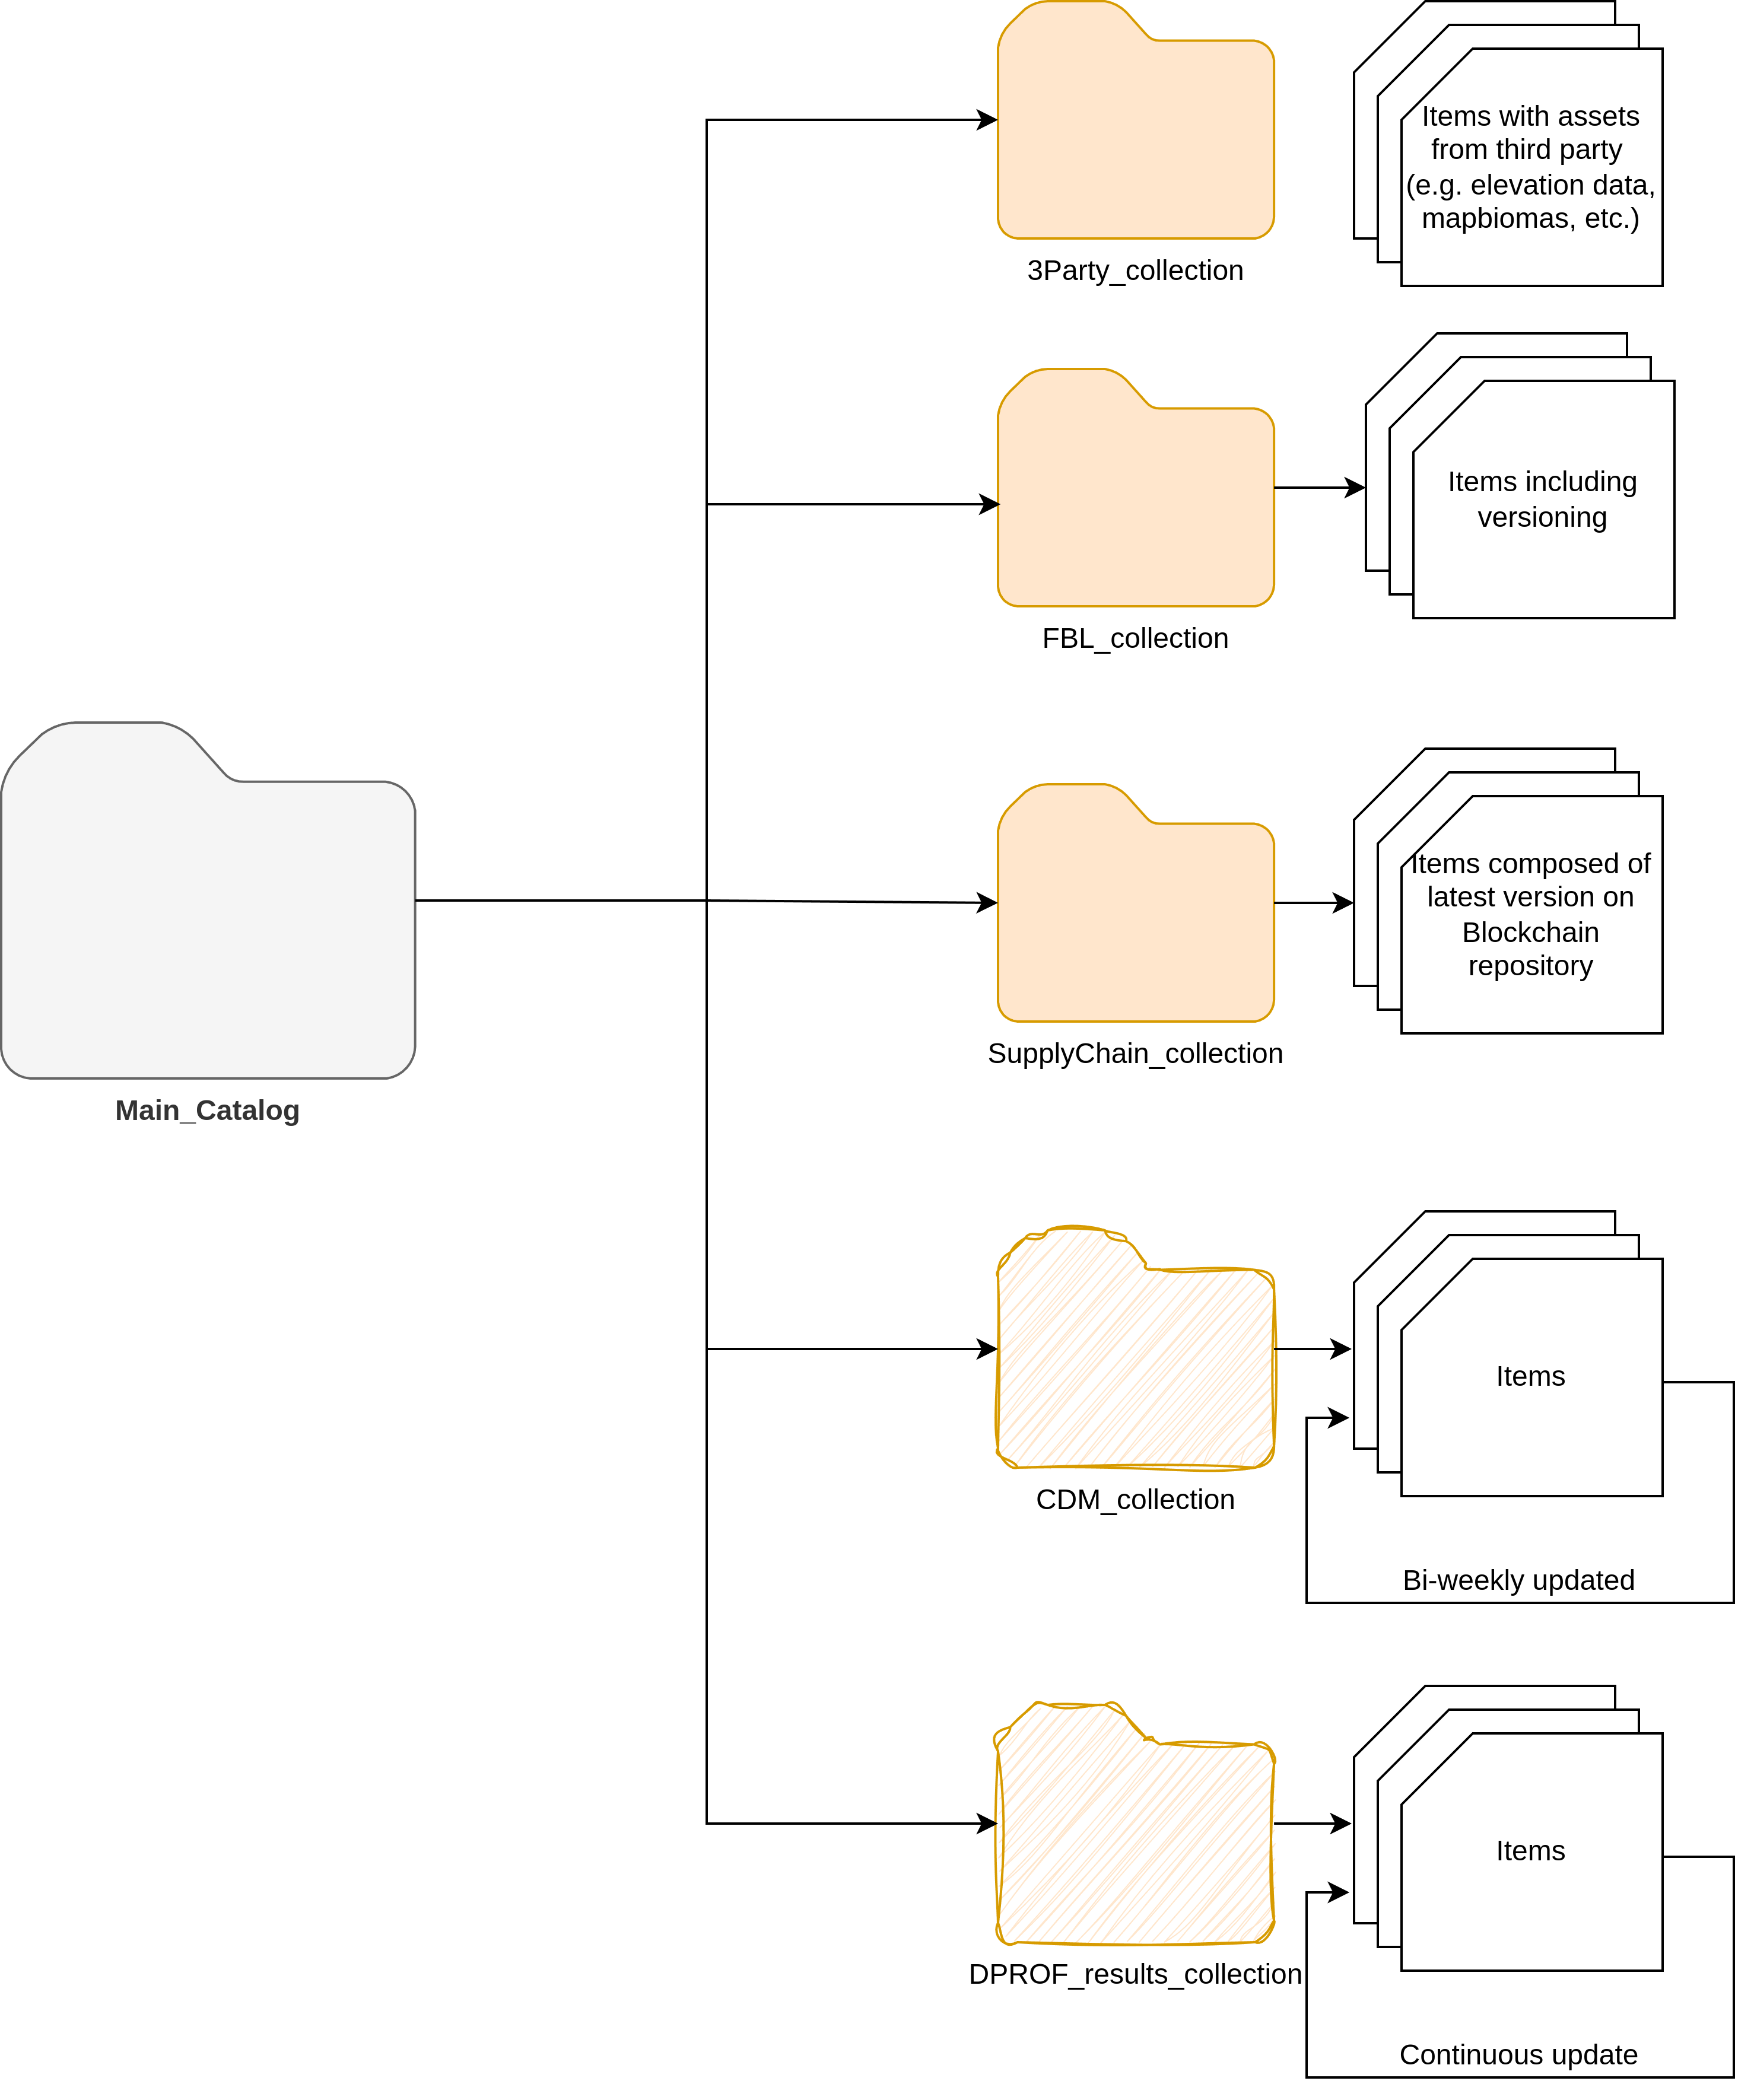
\includegraphics[width=0.9\textwidth,height=\textheight]{img/STAC_Satelligence_structure.png}

}

\caption{\label{fig-stac-str}Proposed STAC structure}

\end{figure}%

\subsection{S11-cats repository}\label{s11-cats-repository}

The \href{https://gitlab.com/satelligence/s11-cats}{s11-cats repository}
created is composed of a module named \texttt{cats} which consists of
five submodules described in Table~\ref{tbl-cats-modules}. Moreover, an
overview of the main workflow followed in the main function of s11-cats
is presented on Figure~\ref{fig-s11-cats}.

\begin{longtable}[]{@{}
  >{\raggedright\arraybackslash}p{(\columnwidth - 2\tabcolsep) * \real{0.4722}}
  >{\raggedright\arraybackslash}p{(\columnwidth - 2\tabcolsep) * \real{0.5278}}@{}}
\caption{Description of cats
submodules}\label{tbl-cats-modules}\tabularnewline
\toprule\noalign{}
\begin{minipage}[b]{\linewidth}\raggedright
\textbf{Submodule}
\end{minipage} & \begin{minipage}[b]{\linewidth}\raggedright
\textbf{Description}
\end{minipage} \\
\midrule\noalign{}
\endfirsthead
\toprule\noalign{}
\begin{minipage}[b]{\linewidth}\raggedright
\textbf{Submodule}
\end{minipage} & \begin{minipage}[b]{\linewidth}\raggedright
\textbf{Description}
\end{minipage} \\
\midrule\noalign{}
\endhead
\bottomrule\noalign{}
\endlastfoot
\emph{gcs\_tools} & Module with functions to interact with data stored
at Google Cloud Storage \\
\emph{general\_metadata} & Module to extract general metadata for a STAC
item. \\
\emph{get\_spatial\_info} & Module to get all spatial information from
assets. \\
\emph{get\_temporal\_info} & Module with functions to extract temporal
metadata of a dataset. \\
\emph{stac\_tools} & Module with the functions to initialize a STAC, add
collections, items and assets to it. \\
\end{longtable}

\begin{figure}[H]

\centering{

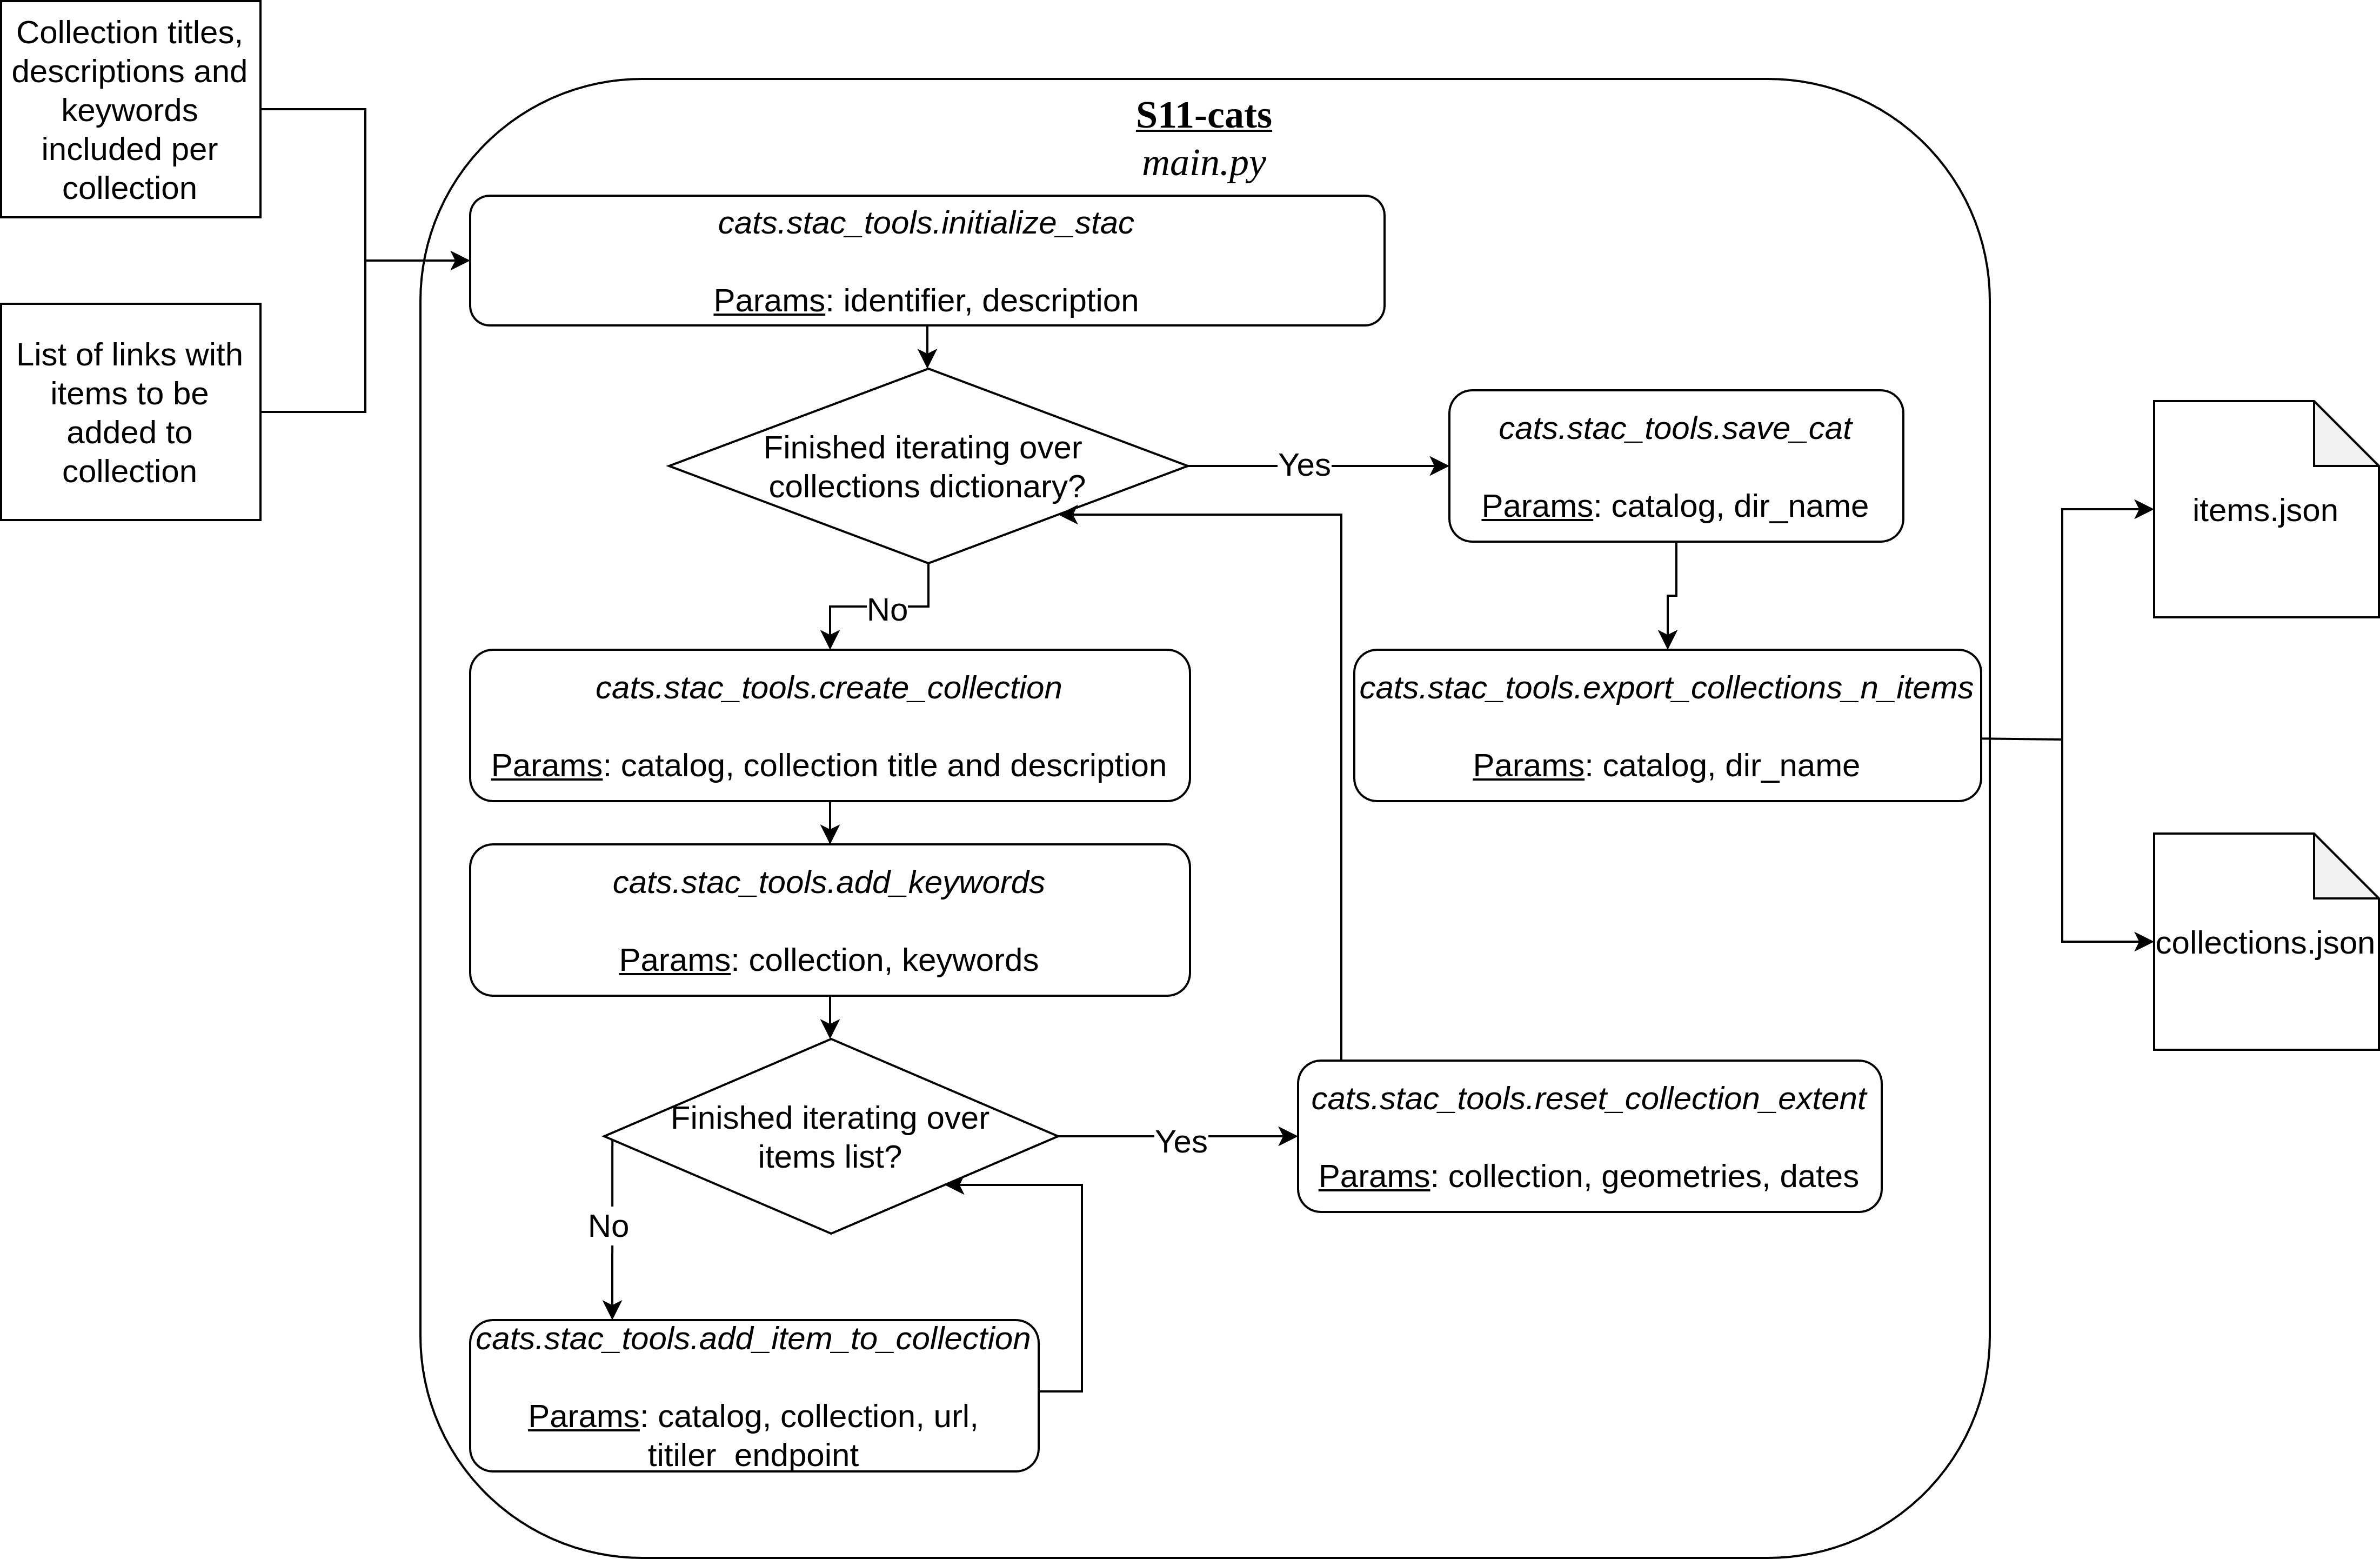
\includegraphics{img/s11-cats.png}

}

\caption{\label{fig-s11-cats}S11- cats main function}

\end{figure}%

As observed, the code in the repository requires a dictionary containing
collection titles, descriptions, and tags, along with a list of links
for each item to be added to each collection. It then generates two JSON
files: one storing the collections' information and the other storing
the items' information. This decision to produce two JSON files was made
to facilitate the transition from the static catalog that has been
created to the dynamic catalog that is desired.

\subsection{eoAPI + other services}\label{sec-eoapi}

Once a static catalog has been created, the next step involves
developing the dynamic catalog by leveraging
\href{https://eoapi.dev/}{eoAPI}
(\citeproc{ref-sarago_developmentseedeoapi_2024}{Sarago et al., 2024}).
\href{https://eoapi.dev/}{eoAPI} is a robust tool designed for managing,
discovering and visualizing Earth observation data. It integrates
several services that include indexing of large STAC collections and
items using a Postgres database (See
\href{https://github.com/stac-utils/pgstac}{PgSTAC}), creating a dynamic
catalog that can query the Postgres database (See
\href{https://github.com/stac-utils/stac-fastapi}{STAC API}) and two
additional services for visualizing raster (See
\href{https://github.com/stac-utils/titiler-pgstac}{Titiler-PgSTAC}) and
vector data (See \href{https://github.com/developmentseed/tipg}{TiPg}).

\href{https://eoapi.dev/}{eoAPI} integrates all of these services by
using containerized versions that are able to communicate seamlessly
with each other. A container is a lightweight, standalone, and
executable package of software that includes everything needed to run an
application. Containerizing the services facilitates deployment to the
cloud using Google Kubernetes Engine (GKE). Kubernetes is an open-source
platform designed for automating the deployment, scaling, and management
of containerized applications
(\citeproc{ref-poulton_kubernetes_2023}{Poulton, 2023}). It offers
various advantages, such as scalability, efficient resource utilization,
and simplified maintenance, making it an ideal solution for managing the
dynamic catalog and the integrated services in a cloud environment.

Since the current version of \href{https://eoapi.dev/}{eoAPI} does not
include some extra services that were necessary to deploy, a separate
containerized version of these services was deployed in the same K8
cluster. Notably, a version of
\href{https://github.com/radiantearth/stac-browser}{STAC Browser} and
\href{https://github.com/developmentseed/titiler-xarray}{TiTiler-Xarray}
to browse the catalog created and visualize Zarr datasets respectively.

\subsection{CI/CD pipeline}\label{cicd-pipeline}

Finally, a gitlab CI/CD pipeline was created to automate the creation of
the catalog using the
\href{https://gitlab.com/satelligence/s11-cats}{s11-cats repository},
the deployment of eoAPI and extra services and the ingestion of the
catalog into the deployed version of the dynamic catalog.

\subsection{Comparison with baseline
scenario}\label{comparison-with-baseline-scenario}

Once a version of all of the services integrated was deployed online,
the ease of discovery and visualization was again qualitatively analyzed
by evaluating the steps processed for both finding and visualizing S11
data. These steps were then represented in a flowchart that could be
compared to the one created on Section~\ref{sec-baseline}.

\section{Multi-format data
visualization}\label{multi-format-data-visualization}

To assess the performance of dynamic tiling services for visualizing
Cloud Optimized GeoTIFFs (COGs) and Zarr data formats, the following
approach was undertaken. Firstly, a COG containing forest baseline
information for the Riau region of Indonesia was used to create a series
of Zarr files, each representing different overviews corresponding to
various zoom levels. This pre-processing step, completed by the company
prior to the study, ensured that the same data was used across both data
formats, allowing for direct comparison. Then, the
\href{https://github.com/developmentseed/titiler-xarray}{TiTiler-Xarray}
service was then customized to work with the specific folder structure
of the ZARR overviews previously created. Moreover, containerized
versions of both
\href{https://github.com/developmentseed/titiler-xarray}{TiTiler-Xarray}
(for Zarr files) and
\href{https://github.com/stac-utils/titiler-pgstac}{TiTiler-PgSTAC} (for
COG files) were locally deployed. The performance was measured by
recording the response times for random tile requests at zoom levels
ranging from 9 to 18. Finally, to mitigate the influence of cached data
on response times, each iteration used a different colormap, with a
total of twelve colormaps employed. This methodology enabled a
systematic evaluation of the performance differences between the two
data formats in a geo-spatial data visualization context.

\subsection{Speed up}\label{speed-up}

The performance of both TiTiler services to dynamically create tiles for
the different data formats was evaluated using the Speed Up metric
proposed in Durbha et al. (\citeproc{ref-durbha_advances_2023}{2023})
(Equation~\ref{eq-speed-up}). In this case, the Speed Up explains how
much did the process of requesting tiles sped up by using a data format
A compared to using a data format B.

\begin{equation}\phantomsection\label{eq-speed-up}{ SpeedUp = \frac{t_{format A}}{t_{format B}} }\end{equation}

\subsection{Zoom level influence}\label{zoom-level-influence}

Finally, the effect of the level of zoom in a web map visualization on
the response times of requesting tiles from the different tiling
services was evaluated by fitting an Ordinary Least Squares (OLS)
univariate linear regression that followed Equation~\ref{eq-lin-reg}.

\begin{equation}\phantomsection\label{eq-lin-reg}{ ResponseTime = \beta_1 \cdot ZoomLevel + \beta_0 + \epsilon }\end{equation}

\chapter{Results \& Discussion}\label{results-discussion}

\section{Baseline scenario}\label{baseline-scenario}

\subsection{Current workflow}\label{current-workflow}

One of the main findings of the interviews was the process followed
currently to discover, retrieve and visualize data. These steps are
summarized on Figure~\ref{fig-baseline} and show how complex and time
consuming these tasks can be for a Satelligence employee nowadays.
Moreover, the steps followed were categorized in four classes depending
on how much time is generally spent carrying it out.

\begin{figure}[H]

\centering{

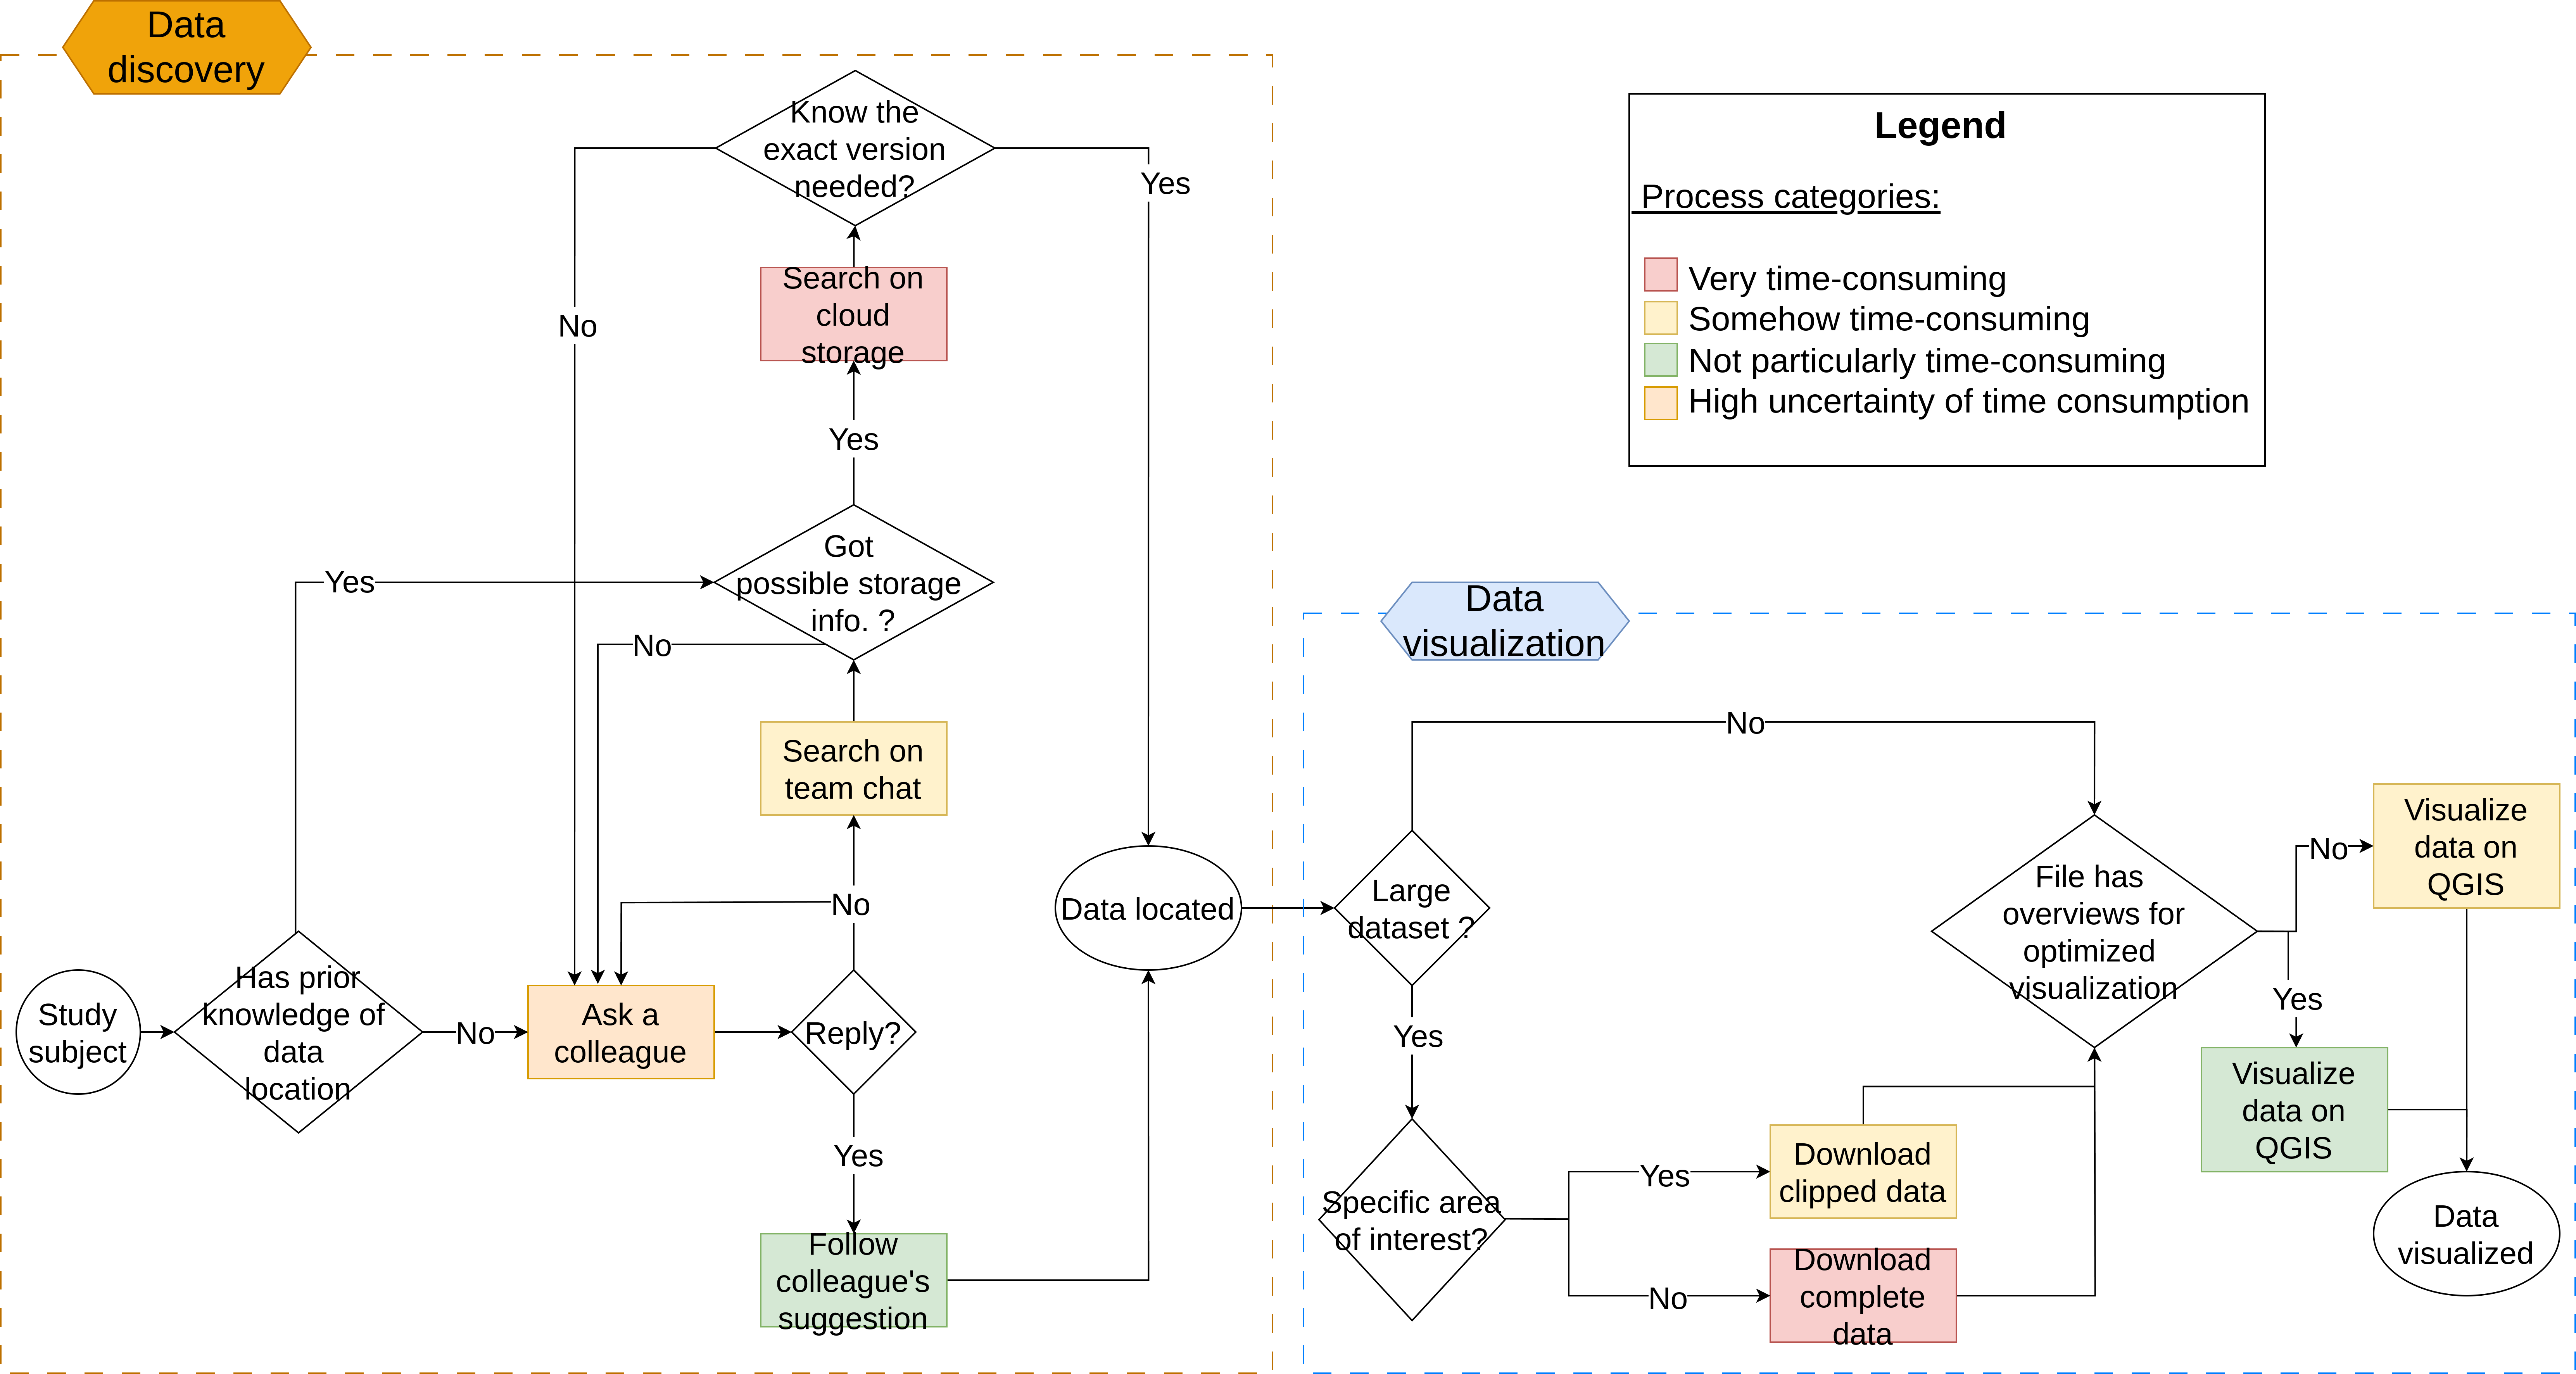
\includegraphics[width=1\textwidth,height=\textheight]{img/Baseline_data_discovery_workflow.png}

}

\caption{\label{fig-baseline}Baseline workflow}

\end{figure}%

According to Figure~\ref{fig-baseline}, some of the most time-consuming
tasks were searching for data on Google Cloud Storage and downloading it
for visualization. Additionally, seeking advice from colleagues about
the dataset's location added a major uncertainty to the time estimates,
as responses varied from very quick to considerably delayed or non
existent.

\subsection{Thematic Content Analysis}\label{thematic-content-analysis}

When asked about the recurrent patterns on the interviews undertaken to
define the baseline scenario, ChatGPT found four main topics:

\begin{itemize}
\tightlist
\item
  There is a high uncertainty on the location of datasets and a high
  dependency on colleagues to find them.
\item
  Multiple sources and locations of data.
\item
  Data familiarity helps users locate data quicker.
\item
  Use of specific tools and methods for different datasets.
\end{itemize}

After some refinement and a deeper analysis of the interviews, the major
pitfalls found on the process of data discovery and visualization in the
company were summarized as follows:

\begin{itemize}
\tightlist
\item
  High dependency on colleagues for dataset location.
\item
  Disorganized structure of Google Storage Buckets.
\item
  Data familiarity helps users locate data quicker.
\item
  Data location is dependent on recurrent work with a specific dataset.
\item
  Not intuitive naming of repositories with datasets.
\item
  Understanding of diverse tools to access different data is currently
  necessary.
\item
  Download of data is required in most cases to visualize it.
\item
  Not one place where all existing data can be found.
\end{itemize}

All of these pitfalls highlight the need for a simpler data discovery
implementation, where data visualization can also be integrated
seamlessly. This approach should allow for easy access to datasets based
on specific queries.

All of these pitfalls highlight the need for a simpler data discovery
implementation, where data visualization can also be integrated
seamlessly. Previous studies have found that key difficulties for earth
observation data discovery include heterogeneous query interfaces, and
use of diverse metadata models
(\citeproc{ref-miranda_espinosa_reviewing_2020}{Miranda Espinosa et al.,
2020}). To address these challenges, the approach should enable easy
access to datasets based on specific queries, ensuring that users can
efficiently locate and utilize the data they need. By harmonizing
metadata standards and query protocols, the process of data discovery
can be greatly improved, making it more accessible and user-friendly.

\section{Service integration}\label{service-integration}

The integration of the services deployed resulted in a version of STAC
Browser including three different collections containing datasets
related to the forest baseline created by the company, elevation data
from third party organizations and a collection for the comparison of
COG and Zarr data. The web application can be accessed in
\href{https://eoapi.satelligence.com/browser/?.language=en}{https://eoapi.satelligence.com/browser}.

\subsection{Effective integration}\label{effective-integration}

The effective integration was not an easy task and involved multiple
aspects, ranging from editing data formats to facilitate their
visualization, transitioning from a static to a dynamic catalog,
customizing APIs, and finalizing with the correct deployment of the
services.

\subsubsection*{Data formats}\label{data-formats}
\addcontentsline{toc}{subsubsection}{Data formats}

An essential step related to data formats was the edition of Zarr
datasets to achieve their optimal visualization. This edition involved
creating a series of overviews of the same dataset at different
resolutions. Specifically, this was accomplished by converting Cloud
Optimized GeoTIFFs (COGs) into multiple Zarr files resampled at various
spatial resolutions. These resampled Zarr files, acting as overviews
enhance visualization by allowing the appropriate resolution to be
accessed based on the map scale, similar to the approach used when
visualizing COGs (\citeproc{ref-lynnes_cloud_2020}{Lynnes et al.,
2020}). Even though the approach followed in this study allowed for
improved visualization of Zarr files, the creation of Zarr pyramids in a
more optimized way is still necessary. Other researchers have been
focusing their efforts on this task to enhance the efficiency and
effectiveness of the process
(\citeproc{ref-Barciauskas_NextGen_2024}{Barciauskas et al., 2024}).

\subsubsection*{Leverage of APIs}\label{leverage-of-apis}
\addcontentsline{toc}{subsubsection}{Leverage of APIs}

To effectively query the datasets stored in the catalog, a transition
from a static to a dynamic catalog (i.e.~a STAC API) was needed. This
shift was facilitated by the deployment of a STAC API within the eoAPI
framework. The STAC API possibilitated the querying capabilities of the
datasets stored in the catalog by dynamically requesting datasets based
on their metadata. This dynamic setup not only facilitated data
discovery but also enabled the use of additional tools such as the STAC
API QGIS plugin. The plugin could simplify the process of data discovery
and its direct manipulation.

For the visualization of Zarr datasets, it was necessary to customize
the TiTiler-Xarray API to accommodate the new Zarr pyramid structure.
This customization involved overwriting a series of functions in the
main code of the application to align with the newly created Zarr
pyramids. By adapting the API to handle the specific requirements of the
Zarr format and its multi-resolution overviews, the visualization
process was optimized.

\subsubsection*{Deployment}\label{deployment}
\addcontentsline{toc}{subsubsection}{Deployment}

As described on Section~\ref{sec-eoapi}, the deployment of both eoAPI
and the additional services utilized was perform using Google Kubernetes
Engine (GKE), which is K8s' GCP service. In a GKE cluster, the setup of
complex multi-service applications that connect to each other with an
internal network is simplified
(\citeproc{ref-gupta_deployment_2021}{Gupta et al., 2021}). Moreover,
\href{www.eoapi.dev}{eoAPI} simplified the deployment by providing a
guide for deployment that used a Helm chart. A Helm chart is a
collection of files that describe the K8s related resources needed to
run a multi-service application and it can improve the speed of
deployment by a factor of up to 6 times
(\citeproc{ref-gokhale_creating_2021}{Gokhale et al., 2021}). These
factors greatly influenced the decision of deploying the whole suite of
services in eoAPI.

Moreover, the performance of some of the eoAPI services deployed using
K8s had been already assessed by previous studies. For instance,
Munteanu et al. (\citeproc{ref-munteanu_performance_2024}{2024})
performed tests on a deployed version of STAC API that, like the
deployment performed in this study, used PgSTAC as the backend. These
authors deployed a dynamic STAC API loaded with the metadata of
approximately 2.3 TB of spatial data on a K8s cluster and evaluated the
performance by assessing both the response times and resources used in a
hypothetical scenario where 7,000 users would perform requests
simultaneously. Their results showed that these services are capable of
supporting effectively a much larger amount of users than the estimated
by Satelligence.

Finally, additional to the already covered advantages, the deployment of
\href{www.eoapi.dev}{eoAPI} and the fast community driven development of
new tools brings with it benefits that could become very important for
S11's workflow. For instance, the visualization of vector data using
\href{https://github.com/developmentseed/tipg}{TiPg} is a service
included in the eoAPI deployment that wasn't used during this
internship, but should certainly be integrated in the near future by the
company to visualize their supply chain datasets. Moroever, the
community adopting STAC specifications has been growing fastly. Due to
this, a big series of STAC-extensions have been developed to fulfill the
requirements of the users. During this internship, extensions to add
additional metadata were included, however, due to time constraints
other extensions that could prove beneficial for the company were not
integrated. Specifically, the possibility of adding an authentication
layer to the catalog still needs to be done and should be the next step
to ensure the privacy of the data.

\subsection{Workflow improvement}\label{workflow-improvement}

Once the deployment of eoAPI and the extra services was done, a new
workflow for both the new data discovery and visualization tasks was
designed and is presented on Figure~\ref{fig-new-workflow}. This new
workflow shows a clear improvement on the speed and the ease of use of
the new methods employed.

\begin{figure}[H]

\centering{

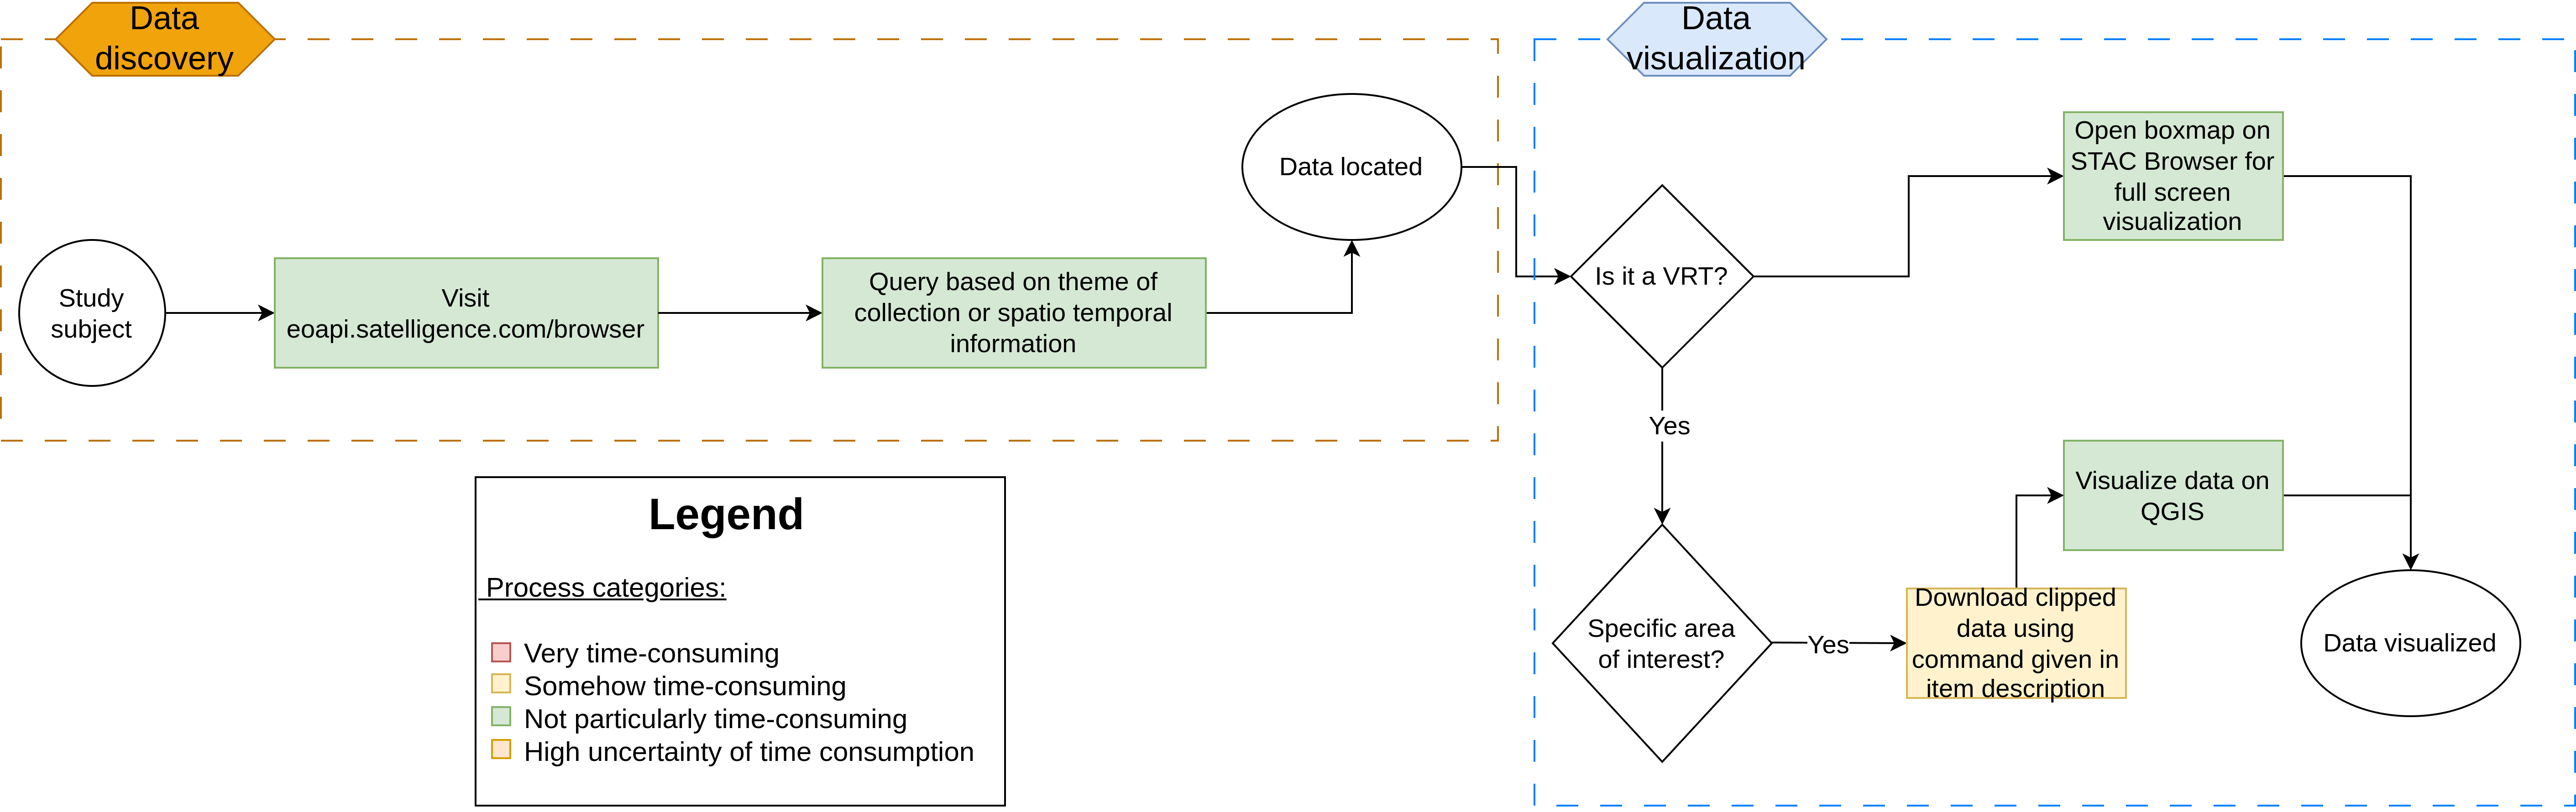
\includegraphics[width=1\textwidth,height=\textheight]{img/New_data_discovery_workflow.png}

}

\caption{\label{fig-new-workflow}New data discovery and visualization
workflow}

\end{figure}%

Moreover, it can be seen that with the new implementation most of the
issues identified on the TCA were addressed. There is no longer a
dependency on colleagues for locating datasets, as all data is now
consolidated in one place. The disorganized structure of Google Storage
Buckets is no longer a concern since the catalog can integrate data
stored in multiple buckets into a single, cohesive STAC collection. The
previous issue of non-intuitive naming conventions for data
repositories, is resolved because it is unnecessary to know the data
source once it is included in the STAC catalog. Furthermore, there is no
longer a need to understand diverse tools for accessing different data;
the STAC Browser facilitates querying collections and visualizing items.
Finally, the STAC catalog serves as the centralized location for all
data used in S11 workflows, which favours long term usability of code
that relies on this data.

\section{Performance of multi-format data
visualization}\label{performance-of-multi-format-data-visualization}

The results of the experiments made with different cloud-optimized data
formats are presented in two subsections. The first subsection evaluates
the overall performance of the two data formats and the second
subsection assess the performance of these data formats based on
different zoom levels.

\subsection{Raster formats}\label{raster-formats}

The comparison of visualization speeds with TiTiler-Xarray for Zarr
datasets and TiTiler-PgSTAC for COGs are presented on
Figure~\ref{fig-format-comp}. In the figure it can be obeserved that on
average the response for requests of COG tiles was 2.53 times faster
than the one for the same file in ZARR format. Moreover,
Figure~\ref{fig-format-comp} shows that the response times for tiles
created from data stored as Zarr showed a considerable wider range than
the ones generated from data in the COG format, which indicates more
variability in the performance for Zarr.

\begin{figure}[H]

\centering{

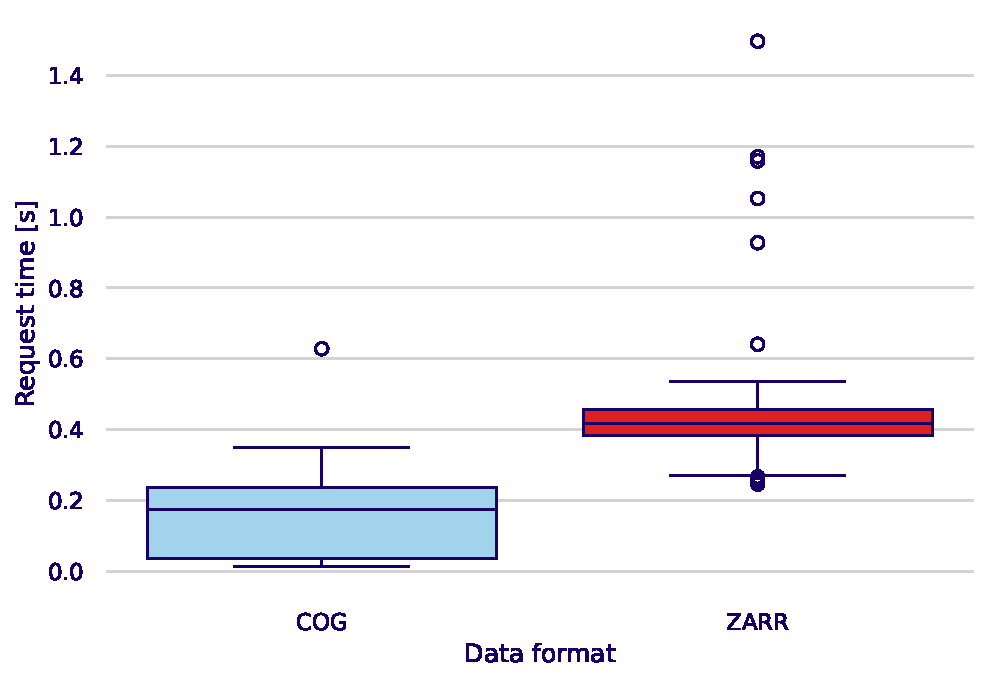
\includegraphics{FinalReport_files/figure-pdf/fig-format-comp-output-1.pdf}

}

\caption{\label{fig-format-comp}Response times for tile requests
depending on data format and zoom level}

\end{figure}%

The results obtained are coherent to the ones previously shown by IMPACT
(\citeproc{ref-nasa_impact_zarr_2023}{2023}), where COGs' rendering time
was found to be lower than the one for Zarr files at different zoom
levels. These results show that COGs, being specifically optimized for
spatial data visualization, offer faster visualization compared to Zarr
files. However, this does not take away from the fact that Zarr provides
additional benefits, such as the ability to store n-dimensional arrays.
Furthermore, recent advancements like GeoZarr and the creation of Zarr
pyramids with new packages like
\href{https://github.com/carbonplan/ndpyramid}{ndpyramid} could bring
significant improvements to this data format Barciauskas et al.
(\citeproc{ref-Barciauskas_NextGen_2024}{2024}).

\subsubsection*{Fine tuning of dataset}\label{fine-tuning-of-dataset}
\addcontentsline{toc}{subsubsection}{Fine tuning of dataset}

Even though COGs showed to be very performant, their performance could
be further enhanced by tuning specific GDAL parameters. These
adjustments could improve the speed of tiling services using COG
(\citeproc{ref-nasa_impact_zarr_2023}{IMPACT, 2023}). Future
considerations should include optimizing these parameters to maximize
efficiency (See
\href{https://developmentseed.org/titiler/advanced/performance_tuning/}{performance
tuning section}).

\subsection{Effects of zoom level}\label{effects-of-zoom-level}

\begin{verbatim}
                            OLS Regression Results                            
==============================================================================
Dep. Variable:                    COG   R-squared:                       0.068
Model:                            OLS   Adj. R-squared:                  0.060
Method:                 Least Squares   F-statistic:                     8.594
Date:                Tue, 30 Jul 2024   Prob (F-statistic):            0.00405
Time:                        07:20:27   Log-Likelihood:                 97.528
No. Observations:                 120   AIC:                            -191.1
Df Residuals:                     118   BIC:                            -185.5
Df Model:                           1                                         
Covariance Type:            nonrobust                                         
==============================================================================
                 coef    std err          t      P>|t|      [0.025      0.975]
------------------------------------------------------------------------------
const          0.3098      0.047      6.524      0.000       0.216       0.404
zoom level    -0.0101      0.003     -2.932      0.004      -0.017      -0.003
==============================================================================
Omnibus:                       15.431   Durbin-Watson:                   1.240
Prob(Omnibus):                  0.000   Jarque-Bera (JB):               25.004
Skew:                           0.596   Prob(JB):                     3.72e-06
Kurtosis:                       4.892   Cond. No.                         66.7
==============================================================================

Notes:
[1] Standard Errors assume that the covariance matrix of the errors is correctly specified.
                            OLS Regression Results                            
==============================================================================
Dep. Variable:                   ZARR   R-squared:                       0.001
Model:                            OLS   Adj. R-squared:                 -0.008
Method:                 Least Squares   F-statistic:                    0.1041
Date:                Tue, 30 Jul 2024   Prob (F-statistic):              0.748
Time:                        07:20:27   Log-Likelihood:                 37.243
No. Observations:                 120   AIC:                            -70.49
Df Residuals:                     118   BIC:                            -64.91
Df Model:                           1                                         
Covariance Type:            nonrobust                                         
==============================================================================
                 coef    std err          t      P>|t|      [0.025      0.975]
------------------------------------------------------------------------------
const          0.4153      0.078      5.292      0.000       0.260       0.571
zoom level     0.0018      0.006      0.323      0.748      -0.009       0.013
==============================================================================
Omnibus:                      126.673   Durbin-Watson:                   1.460
Prob(Omnibus):                  0.000   Jarque-Bera (JB):             1844.290
Skew:                           3.780   Prob(JB):                         0.00
Kurtosis:                      20.655   Cond. No.                         66.7
==============================================================================

Notes:
[1] Standard Errors assume that the covariance matrix of the errors is correctly specified.
\end{verbatim}

As seen on Figure~\ref{fig-comp-zoom}, the zoom level of the map showed
an effect on the time spent requesting and getting a tile from a tiling
service for the COG format. In this study, it was found that the request
times decreased by -0.01 seconds per zoom level for COGs, and didn't
show a notable change for Zarrs (0.002 seconds per zoom level). The
behaviour presented here for COGs differs from the one observed by
IMPACT (\citeproc{ref-nasa_impact_zarr_2023}{2023}), where no difference
in rendering time was observed as a function of the zoom level. This
difference could be explained by the fact that in their study, only the
lowest zoom levels were considered, while in this study only the highest
zoom levels were taken into account, however, to verify this hypothesis
a broader study of the response times at more zoom levels should be
performed. This was not done in this study because the limited size of
the study area that the raster images covered only allowed visualization
of the data at high zoom levels (i.e., above 8).

\begin{figure}[H]

\centering{

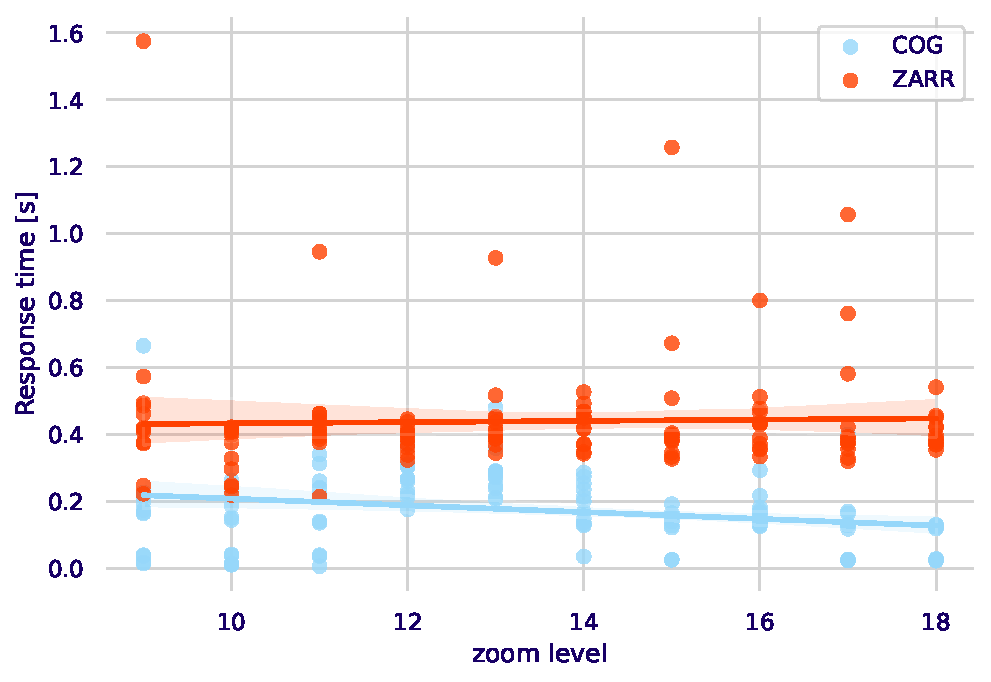
\includegraphics{FinalReport_files/figure-pdf/fig-comp-zoom-output-1.pdf}

}

\caption{\label{fig-comp-zoom}Request times depending on zoom level and
their respective trends for COG and Zarr data formats.}

\end{figure}%

Moreover, as seen on Figure~\ref{fig-chunksize-zarr}, while the size of
blocks remain constant throughout all of the overviews in the COG file,
the sizes of the Zarr chunks varied in the pyramids created. Due to
this, the tiles requested at higher zoom levels were larger than the
ones requested at lower zoom levels which could explain the difference
between the trends observed in Figure~\ref{fig-comp-zoom} for the two
data formats.

\begin{figure}[H]

\centering{

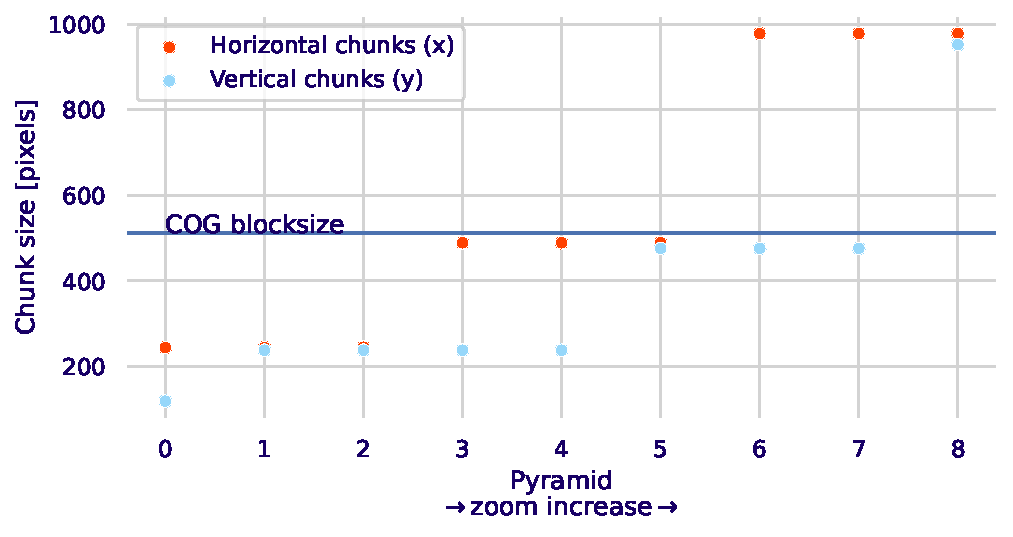
\includegraphics{FinalReport_files/figure-pdf/fig-chunksize-zarr-output-1.pdf}

}

\caption{\label{fig-chunksize-zarr}Variation of chunk sizes in Zarr file
depending on zoom level compared to a constant block size for COG data
format.}

\end{figure}%

\chapter{Conclusions}\label{conclusions}

The conclusions of the work performed during this internship are
presented below in relationship to each research question:

\begin{itemize}
\tightlist
\item
  \textbf{\emph{What are the current challenges, practices, and user
  experiences related to data discovery and data visualization in the
  company?}}
\end{itemize}

The qualitative analysis of the current workflow at Satelligence
revealed a complex and time-consuming process for data discovery,
retrieval, and visualization. Major inefficiencies identified by the TCA
included high dependency on colleagues for locating datasets, a
disorganized structure of Google Storage Buckets and the need to
download full datasets for visualization. The challenges found
underscore the necessity for a user-friendly data discovery
implementation where data visualization can also be integrated.

\begin{itemize}
\tightlist
\item
  \textbf{\emph{How can cloud-optimized data formats, cloud services and
  SpatioTemporal Asset Catalog (STAC) specifications be integrated to
  enhance the process and experiences of discovering and visualizing big
  spatial data within the company?}}
\end{itemize}

The integration of cloud-optimized data formats, cloud services, and
SpatioTemporal Asset Catalog (STAC) specifications has greatly enhanced
data discovery and visualization for Satelligence. Despite the
challenges that could be involved in integrating these aspects, this
study presents a methodology that leverages customized cloud optimized
data formats, the integration of several services (i.e.~eoAPI, STAC
Browser and TiTiler-Xarray), and the deployment on GKE to achieve
effective integration. The solution proposed her addresses challenges
found previously. Finally, the consolidation of all data in one place
ensures long-term usability and an easier management of big spatial
data.

\begin{itemize}
\tightlist
\item
  \textbf{\emph{To what extent do dynamic tiling services perform in
  visualizing different cloud-optimized data formats?}}
\end{itemize}

Dynamic tiling services vary in performance when visualizing different
cloud-optimized data-formats. In this study, the performance evaluation
showed that COG tiles were, on average, 2.53 times faster to be
requested than Zarr tiles, with less variability in response times.
These results align with the understanding that COGs are specifically
optimized for spatial data visualization, whereas Zarrs are not.
Although this study made efforts to improve Zarr visualization using
customized pyramids, recent advancements such as GeoZarr and more
efficient Zarr pyramids generation could further enhance Zarr
visualization performance.

\chapter*{References}\label{references}
\addcontentsline{toc}{chapter}{References}

\phantomsection\label{refs}
\begin{CSLReferences}{1}{0}
\bibitem[\citeproctext]{ref-anderson_thematic_2007}
Anderson, R. (2007). \emph{Thematic content analysis ({TCA})}.
\url{https://rosemarieanderson.com/wp-content/uploads/2014/08/ThematicContentAnalysis.pdf}

\bibitem[\citeproctext]{ref-Barciauskas_NextGen_2024}
Barciauskas, A., Jones, M., Martin, K., Harkins, S. and Sarago, V.
(2024). {Next-Gen Zarr Web Map Visualization}. \emph{EGU General
Assembly Conference Abstracts}, 11805. p.
\url{https://doi.org/10.5194/egusphere-egu24-11805}

\bibitem[\citeproctext]{ref-brodeur_geographic_2019}
Brodeur, J., Coetzee, S., Danko, D., Garcia, S. and Hjelmager, J.
(2019). Geographic information metadata---an outlook from the
international standardization perspective. \emph{{ISPRS} International
Journal of Geo-Information}, \emph{8}(6), 280. p.
\url{https://doi.org/10.3390/ijgi8060280}

\bibitem[\citeproctext]{ref-chester_ogc_2024}
Chester, S. (2024(e)ko Januaryk 18). \emph{{OGC} forms new {GeoZarr}
standards working group to establish a zarr encoding for geospatial
data. Open geospatial consortium}.
\url{https://www.ogc.org/press-release/ogc-forms-new-geozarr-standards-working-group-to-establish-a-zarr-encoding-for-geospatial-data/}

\bibitem[\citeproctext]{ref-clark_api_2020}
Clark, J. (2020). \emph{Application programming interface}.
\href{https://www.semanticscholar.org/\%20paper/Application-Programming-Interface-Clark/84f0b513a62a4f2bb09a899a128a231\%20eccace22c}{https://www.semanticscholar.org/
paper/Application-Programming-Interface-Clark/84f0b513a62a4f2bb09a899a128a231
eccace22c}

\bibitem[\citeproctext]{ref-desruisseaux_ogc_2021}
Desruisseaux, M., Giacco, G., Goncalves, P., Manente, M. and Rouault, E.
(2021). \emph{{OGC} testbed 17: {COG}/zarr evaluation engineering
report}. \url{https://docs.ogc.org/per/21-032.html\#toc11}

\bibitem[\citeproctext]{ref-durbha_advances_2023}
Durbha, S. S., Sanyal, J., Yang, L., S Chaudhari, S., Bhangale, U.,
Bharambe, U. and Kurte, K. (2023). \emph{Advances in scalable and
intelligent geospatial analytics: Challenges and applications} (1st
ed.). {CRC} Press. \url{https://doi.org/10.1201/9781003270928}

\bibitem[\citeproctext]{ref-giri_big_2014}
Giri, K. and Lone, T. (2014). Big data -overview and challenges.
\emph{International Journal of Advanced Research in Computer Science and
Software Engineering}, \emph{4}.

\bibitem[\citeproctext]{ref-gokhale_creating_2021}
Gokhale, S., Poosarla, R., Tikar, S., Gunjawate, S., Hajare, A.,
Deshpande, S., Gupta, S. and Karve, K. (2021). Creating helm charts to
ease deployment of enterprise application and its related services in
kubernetes. \emph{2021 International Conference on Computing,
Communication and Green Engineering ({CCGE})}, 1--5. pp.
\url{https://doi.org/10.1109/CCGE50943.2021.9776450}

\bibitem[\citeproctext]{ref-gupta_deployment_2021}
Gupta, M., Sanjana, K., Akhilesh, K. and Chowdary, M. N. (2021).
Deployment of multi-tier application on cloud and continuous monitoring
using kubernetes. \emph{2021 5th International Conference on Electrical,
Electronics, Communication, Computer Technologies and Optimization
Techniques ({ICEECCOT})}, 602--607. pp.
\url{https://doi.org/10.1109/ICEECCOT52851.2021.9707957}

\bibitem[\citeproctext]{ref-holmes_spatiotemporal_2021}
Holmes, C. (2021(e)ko Januaryk 19). \emph{{SpatioTemporal} asset
catalogs and the open geospatial consortium. Radiant earth insights}.
\url{https://medium.com/radiant-earth-insights/spatiotemporal-asset-catalogs-and-the-open-geospatial-consortium-659538dce5c7}

\bibitem[\citeproctext]{ref-nasa_impact_zarr_2023}
IMPACT, N. (2023). \emph{Zarr visualization report}. Nasa.
\url{https://nasa-impact.github.io/zarr-visualization-report/}

\bibitem[\citeproctext]{ref-kaufmann_database_2023}
Kaufmann, M. and Meier, A. (2023). Database management. In M. Kaufmann
and A. Meier (Eds.), \emph{{SQL} and {NoSQL} databases: Modeling,
languages, security and architectures for big data management} (1--24.
pp.). Springer Nature Switzerland.
\url{https://doi.org/10.1007/978-3-031-27908-9_1}

\bibitem[\citeproctext]{ref-lynnes_cloud_2020}
Lynnes, C., Quinn, P., Durbin, C. and Shum, D. (2020). \emph{Cloud
optimized data formats}.

\bibitem[\citeproctext]{ref-miranda_espinosa_reviewing_2020}
Miranda Espinosa, M. T., Giuliani, G. and Ray, N. (2020). Reviewing the
discoverability and accessibility to data and information products
linked to essential climate variables. \emph{International Journal of
Digital Earth}, \emph{13}(2), 236--252. pp.
\url{https://doi.org/10.1080/17538947.2019.1620882}

\bibitem[\citeproctext]{ref-mishra_structured_2017}
Mishra, S. and Misra, A. (2017). Structured and unstructured big data
analytics. \emph{2017 International Conference on Current Trends in
Computer, Electrical, Electronics and Communication ({CTCEEC})},
740--746. pp. \url{https://doi.org/10.1109/CTCEEC.2017.8454999}

\bibitem[\citeproctext]{ref-munteanu_performance_2024}
Munteanu, A., Panica, S. and Iuhasz, G. (2024). On the performance of
{STAC}-{FastAPI} and {PgSTAC} using a cloud-native deployment. In L.
Barolli (Ed.), \emph{Advanced information networking and applications}
(191--200. pp.). Springer Nature Switzerland.
\url{https://doi.org/10.1007/978-3-031-57931-8_19}

\bibitem[\citeproctext]{ref-ogc_ogc_2023}
OGC. (2023). \emph{{OGC} cloud optimized {GeoTIFF} standard}.
\url{https://docs.ogc.org/is/21-026/21-026.html}

\bibitem[\citeproctext]{ref-openai_chatgpt_2023}
OpenAI. (2023). \emph{{ChatGPT}}. \url{https://chatgpt.com/}

\bibitem[\citeproctext]{ref-pagan_current_2023}
Pagán, B. R., Abernathey, R., Blodgett, D. L., Davis, E., Erickson, T.,
Hanson, M., Harkins, S., Noel, C., Kapadia, A. and Shiklomanov, A. N.
(2023). \emph{Current status of the {GeoZarr} steering working group}.
\emph{2023}, IN34A--04. pp.
\url{https://ui.adsabs.harvard.edu/abs/2023AGUFMIN34A..04P}

\bibitem[\citeproctext]{ref-poulton_kubernetes_2023}
Poulton, N. (2023). \emph{The kubernetes book}. Nigel Poulton Ltd.

\bibitem[\citeproctext]{ref-noauthor_stac-specbest-practicesmd_nodate}
RadiantEarth. (2024). \emph{Stac-spec/best-practices.md at master ·
radiantearth/stac-spec. {GitHub}}.
\url{https://github.com/radiantearth/stac-spec/blob/master/best-practices.md}

\bibitem[\citeproctext]{ref-rajabifard_spatial_2001}
Rajabifard, A. and Williamson, I. P. (2001). \emph{Spatial data
infrastructures: Concept, {SDI} hierarchy and future directions}.
\url{http://hdl.handle.net/11343/33897}

\bibitem[\citeproctext]{ref-sarago_developmentseedeoapi_2024}
Sarago, V., Deziel, Z., Tenezakis, E. and Goodman, L. (2024).
\emph{Developmentseed/{eoAPI}} {[}Software{]}. Development Seed.
\url{https://github.com/developmentseed/eoAPI}

\bibitem[\citeproctext]{ref-satelligence_home_nodate}
Satelligence. (n.d.). \emph{Home - satelligence - sustainability
monitoring simplified. Satelligence}. Retrieved February 5, 2024, from
\url{https://satelligence.com/}

\bibitem[\citeproctext]{ref-satelligence_internship_2023}
Satelligence. (2023). \emph{Internship: Cataloguing and visualizing big
geodata}.

\bibitem[\citeproctext]{ref-noauthor_titiler_nodate}
\emph{{TiTiler}}. (n.d.). Retrieved February 19, 2024, from
\url{https://developmentseed.org/titiler/}

\bibitem[\citeproctext]{ref-tripathi_cloud_2020}
Tripathi, A. K., Agrawal, S. and Gupta, R. D. (2020). Cloud enabled
{SDI} architecture: A review. \emph{Earth Science Informatics},
\emph{13}(2), 211--231. pp.
\url{https://doi.org/10.1007/s12145-020-00446-9}

\bibitem[\citeproctext]{ref-zhao_scalable_2021}
Zhao, Y., Yang, X. and Vatsavai, R. R. (2021). A scalable system for
searching large-scale multi-sensor remote sensing image collections.
\emph{2021 {IEEE} International Conference on Big Data (Big Data)},
3780--3783. pp. \url{https://doi.org/10.1109/BigData52589.2021.9671679}

\end{CSLReferences}

\chapter{Appendix}\label{appendix}

\section{Baseline scenario questionnaire}\label{sec-baseline-q}

\subsection*{Related to data discovery}\label{related-to-data-discovery}
\addcontentsline{toc}{subsection}{Related to data discovery}

\begin{itemize}
\tightlist
\item
  I am working for Wilmar in South East Asia. Do you know what is the
  forest baseline that I should use and where can I find it?
\item
  I have been checking the results of the Soy map we created. Do you
  know which DEM was used for it? And where can I find it?
\item
  Do you know which DEM is used as the terrain mask when using Sentinel
  1 data?
\item
  I need to access the concessions data provided by Grepalma. Where can
  I find it?
\end{itemize}

\subsection*{Related to data
visualization}\label{related-to-data-visualization}
\addcontentsline{toc}{subsection}{Related to data visualization}

\begin{itemize}
\tightlist
\item
  I am interested on getting an overview of where was the primary forest
  present in Colombia in 2007. Could you visualize a layer with this
  data for me?
\item
  I need to visualize the concessions provided by fedepalma. Could you
  do it for me?
\end{itemize}

\section{Thematic Content Analysis prompt}\label{sec-gpt-prompt}

\begin{verbatim}
I will give you some notes I took from an interview I did to four study subjects:
W, X, Y and Z.

Tell me if you identify any themes or topics that are repeated in the notes that 
I took from the answers of the individuals. In other words, do a simple Thematic
Content Analysis of the interviews.
\end{verbatim}

\section{Code to evaluate request times}\label{sec-request-code}

\textbf{Disclaimer:} In order to run the code presented below, the user
must have authenticated their Google account and have the TiTiler-PgSTAC
and the TiTiler-Xarray services running on \texttt{localhost:8082} and
\texttt{localhost:8084} respectively.

\begin{Shaded}
\begin{Highlighting}[]
\ImportTok{import}\NormalTok{ pandas }\ImportTok{as}\NormalTok{ pd}
\ImportTok{import}\NormalTok{ requests}
\ImportTok{import}\NormalTok{ random}

\NormalTok{tiles }\OperatorTok{=}\NormalTok{ [}\StringTok{"6/50/32"}\NormalTok{, }\StringTok{"7/99/63"}\NormalTok{, }\StringTok{"8/199/126"}\NormalTok{, }\StringTok{"9/399/254"}\NormalTok{, }\StringTok{"10/800/505"}\NormalTok{, }\StringTok{"11/1603/1012"}\NormalTok{,  }\StringTok{"12/3209/2042"}\NormalTok{, }
\StringTok{"13/6407/4075"}\NormalTok{, }\StringTok{"14/12817/8159"}\NormalTok{, }\StringTok{"15/25678/16271"}\NormalTok{, }\StringTok{"16/51268/32552"}\NormalTok{, }
\StringTok{"17/102503/65134"}\NormalTok{, }\StringTok{"18/205062/130211"}\NormalTok{]}

\CommentTok{\# Tiles are slightly modified to try to avoid getting cached tiles}
\KeywordTok{def}\NormalTok{ modify\_tile(tile):}
\NormalTok{    parts }\OperatorTok{=}\NormalTok{ tile.split(}\StringTok{\textquotesingle{}/\textquotesingle{}}\NormalTok{)}
\NormalTok{    z }\OperatorTok{=} \BuiltInTok{int}\NormalTok{(parts[}\DecValTok{0}\NormalTok{])}
\NormalTok{    x }\OperatorTok{=} \BuiltInTok{int}\NormalTok{(parts[}\DecValTok{1}\NormalTok{])}
\NormalTok{    y }\OperatorTok{=} \BuiltInTok{int}\NormalTok{(parts[}\DecValTok{2}\NormalTok{])}

    \CommentTok{\# Determine the range of change based on the value of z}
    \ControlFlowTok{if}\NormalTok{ z }\OperatorTok{\textless{}=} \DecValTok{7}\NormalTok{:}
\NormalTok{        change\_range }\OperatorTok{=} \DecValTok{1}
    \ControlFlowTok{elif}\NormalTok{ z }\OperatorTok{\textless{}=} \DecValTok{9}\NormalTok{:}
\NormalTok{        change\_range }\OperatorTok{=} \DecValTok{5}
    \ControlFlowTok{elif}\NormalTok{ z }\OperatorTok{\textless{}=} \DecValTok{12}\NormalTok{:}
\NormalTok{        change\_range }\OperatorTok{=} \DecValTok{5}
    \ControlFlowTok{elif}\NormalTok{ z }\OperatorTok{\textless{}=} \DecValTok{15}\NormalTok{:}
\NormalTok{        change\_range }\OperatorTok{=} \DecValTok{10}
    \ControlFlowTok{elif}\NormalTok{ z }\OperatorTok{\textless{}=} \DecValTok{18}\NormalTok{:}
\NormalTok{        change\_range }\OperatorTok{=} \DecValTok{50}

    \CommentTok{\# Apply the change to x and y}
\NormalTok{    x\_change }\OperatorTok{=}\NormalTok{ random.randint(}\OperatorTok{{-}}\NormalTok{change\_range, change\_range)}
\NormalTok{    y\_change }\OperatorTok{=}\NormalTok{ random.randint(}\OperatorTok{{-}}\NormalTok{change\_range, change\_range)}

\NormalTok{    new\_x }\OperatorTok{=}\NormalTok{ x }\OperatorTok{+}\NormalTok{ x\_change}
\NormalTok{    new\_y }\OperatorTok{=}\NormalTok{ y }\OperatorTok{+}\NormalTok{ y\_change}

    \CommentTok{\# Return the modified tile as a string}
    \ControlFlowTok{return} \SpecialStringTok{f"}\SpecialCharTok{\{}\NormalTok{z}\SpecialCharTok{\}}\SpecialStringTok{/}\SpecialCharTok{\{}\NormalTok{new\_x}\SpecialCharTok{\}}\SpecialStringTok{/}\SpecialCharTok{\{}\NormalTok{new\_y}\SpecialCharTok{\}}\SpecialStringTok{"}

\NormalTok{times\_zarr }\OperatorTok{=}\NormalTok{ []}
\NormalTok{times\_cog }\OperatorTok{=}\NormalTok{ []}
\NormalTok{z\_level }\OperatorTok{=}\NormalTok{ []}
\NormalTok{cmap\_picked }\OperatorTok{=}\NormalTok{ []}

\CommentTok{\# The colormaps picked can be either a customized one for S11}
\CommentTok{\# Forest baseline or greens\_r}
\NormalTok{cmap }\OperatorTok{=}\NormalTok{ [}\StringTok{"\_name=greens\&rescale=0,70"}\NormalTok{,}\StringTok{"\_name=greens\_r\&rescale=0,70"}\NormalTok{,}
        \StringTok{"\_name=blues\&rescale=0,90"}\NormalTok{, }\StringTok{"\_name=blues\_r\&rescale=0,90"}\NormalTok{,}
        \StringTok{"\_name=reds\&rescale=0,80"}\NormalTok{, }\StringTok{"\_name=reds\_r\&rescale=0,80"}\NormalTok{,}
        \StringTok{"\_name=gray\&rescale=0,70"}\NormalTok{,}\StringTok{"\_name=gray\_r\&rescale=0,70"}\NormalTok{,}
        \StringTok{"\_name=jet\&rescale=0,90"}\NormalTok{, }\StringTok{"\_name=jet\_r\&rescale=0,90"}\NormalTok{,}
        \StringTok{"\_name=hot\&rescale=0,80"}\NormalTok{, }\StringTok{"\_name=hot\_r\&rescale=0,80"}\NormalTok{]}

\ControlFlowTok{for}\NormalTok{ i }\KeywordTok{in} \BuiltInTok{range}\NormalTok{(}\BuiltInTok{len}\NormalTok{(cmap)):}

\NormalTok{    mod\_tiles }\OperatorTok{=}\NormalTok{ [modify\_tile(tile) }\ControlFlowTok{for}\NormalTok{ tile }\KeywordTok{in}\NormalTok{ tiles]}
\NormalTok{    k }\OperatorTok{=}\NormalTok{ i}

    \ControlFlowTok{for}\NormalTok{ tile }\KeywordTok{in}\NormalTok{ mod\_tiles:}
\NormalTok{        url\_zarr }\OperatorTok{=} \StringTok{"https://localhost:8084/tiles/WebMercatorQuad/"}\OperatorTok{+\textbackslash{}}
        \SpecialStringTok{f"}\SpecialCharTok{\{}\NormalTok{tile}\SpecialCharTok{\}}\SpecialStringTok{\%401x?url=gs://s11{-}tiles/zarr/separate\&"}\OperatorTok{+\textbackslash{}}
        \StringTok{"variable=band\_data\&reference=false\&decode\_times=true\&"}\OperatorTok{+\textbackslash{}}
        \SpecialStringTok{f"consolidated=true\&colormap}\SpecialCharTok{\{}\NormalTok{cmap[k]}\SpecialCharTok{\}}\SpecialStringTok{\&return\_mask=true"}

\NormalTok{        url\_cog }\OperatorTok{=} \SpecialStringTok{f"https://localhost:8082/collections/"}\OperatorTok{+\textbackslash{}}
        \SpecialStringTok{f"Example\%20FBL\%20Riau/items/FBL\_V5\_2021\_Riau\_cog/tiles/"}\OperatorTok{+\textbackslash{}}
        \SpecialStringTok{f"WebMercatorQuad/}\SpecialCharTok{\{}\NormalTok{tile}\SpecialCharTok{\}}\SpecialStringTok{\%401x?bidx=1\&assets=data\&"}\OperatorTok{+\textbackslash{}}
        \StringTok{"unscale=false\&resampling=nearest\&reproject=nearest\&"}\OperatorTok{+\textbackslash{}}
        \SpecialStringTok{f"colormap}\SpecialCharTok{\{}\NormalTok{cmap[k]}\SpecialCharTok{\}}\SpecialStringTok{\&return\_mask=true"}

\NormalTok{        x }\OperatorTok{=}\NormalTok{ requests.get(url\_zarr)}
\NormalTok{        times\_zarr.append(x.elapsed.total\_seconds())}

\NormalTok{        x }\OperatorTok{=}\NormalTok{ requests.get(url\_cog)}
\NormalTok{        times\_cog.append(x.elapsed.total\_seconds())}

\NormalTok{        z\_level.append(}\BuiltInTok{int}\NormalTok{(tile.split(}\StringTok{\textquotesingle{}/\textquotesingle{}}\NormalTok{)[}\DecValTok{0}\NormalTok{]))}

\NormalTok{        cmap\_picked.append(k)}

\NormalTok{data }\OperatorTok{=}\NormalTok{ pd.DataFrame([cmap\_picked, z\_level, times\_cog, times\_zarr]).T}
\NormalTok{data.columns }\OperatorTok{=}\NormalTok{ [}\StringTok{\textquotesingle{}colormap\textquotesingle{}}\NormalTok{,}\StringTok{\textquotesingle{}zoom level\textquotesingle{}}\NormalTok{,}\StringTok{\textquotesingle{}COG\textquotesingle{}}\NormalTok{, }\StringTok{\textquotesingle{}ZARR\textquotesingle{}}\NormalTok{]}

\NormalTok{data.to\_csv(}\StringTok{\textquotesingle{}request\_time\_results\_6iter\_k8.csv\textquotesingle{}}\NormalTok{)}
\end{Highlighting}
\end{Shaded}



\backmatter

\end{document}
